\documentclass[aspectratio=169, xcolor=table]{beamer}
%% Choose aspect ratio and other standard options:
% [aspectratio=169] % 16:9 (default)
% [aspectratio=43]  % 4:3 

\usetheme[standard]{tugraz2018}
%% Choose main theme variant:
% [standard]        % standard (default)
% [institute]       % with institute's graphical acronym on the left
% [minimal]         % with reduced visuals

%% Choose your font style:
%                   % Helvetica (default for Corporate Design)
% [webfont]         % Source Sans Pro (as used on tugraz.at)
% [nofont]          % no font loaded - Computer Modern Sans

%% For more options, see README.pdf

\usepackage[utf8]{inputenc}
\usepackage[english]{babel}
%% Choose your main language:
% [ngerman]   % German
% [english]   % English


%% Add your own packages, macros, etc.
% tikz
\usepackage{tikz, wrapfig}
\usetikzlibrary{positioning, calc, shapes.geometric, automata}
\usepackage{listings}

\lstset{ 
	tabsize=2, 
	showspaces=false, 
	showstringspaces=false, 
	backgroundcolor=\color{lightgray}, 
	float=[htb], 
	captionpos=b, 
	basicstyle=\footnotesize, 
	frame=tbrl, %t: top, r, b, l 
	frameround=tttt, 
	numbers=none, 
	numberstyle=\tiny, 
	numberblanklines=false, 
	linewidth=.99\textwidth,
	xleftmargin=0.15cm,
	basicstyle=\footnotesize,
	columns=flexible
} 

% grafix


%% Enter presentation metadata
\title[Model Learning and Fuzzing of the IPsec-IKEv1 VPN Protocol]{Model Learning and Fuzzing of the \\ IPsec-IKEv1 VPN Protocol}
\author{Benjamin Wunderling}
\date{Master's Examination 19.10.2023}
\institute{}
\instituteurl{benjamin.wunderling@student.tugraz.at}

%% Logos
% \institutelogo{beamerthemetugraz/institute/kurz}  % graphical acronym for [institute] theme (left margin)
% \additionallogo{figures/logo}  % additional institute/department logo (footline; optional)
% \logobar{Supported by: ...}  % sponsors (titlepage; optional)


\begin{document}

\begin{frame}[plain]
  \maketitle
\end{frame}


\begin{frame}{Outline}
  \vspace{-1.5em}
  \tableofcontents
\end{frame}


\section{Introduction}

\begin{frame}{Motivation}
	\vspace{-1.5em}
	\begin{columns}[T]
		\begin{column}{0.6\textwidth}
			\begin{itemize}
				\item Increased VPN usage
				\pause
				\item IPsec IKEv1 vs IKEv2 (FRITZ!Box)
				\pause
				\item Security testing
				\pause
				\item Behavioral models
				\pause
				\item Black-box systems
			\end{itemize}
		\end{column}
		\begin{column}{0.4\textwidth}
			
\includegraphics[width=1.0\textwidth]{images/vpn.jpg}
			\tikz[overlay, remember picture,
			shift=(current page.south west),
			x=(current page.south east), y=(current page.north west),
			]{
				\node[align=left]at (0.75,0.1) {\tiny \url{https://pixabay.com/photos/personal-data-personal-security-4667362}}; 
				% Optional help grid lines
				%\draw[step=.1, opacity=0.3, thick, red] (0,0) grid (1,1);
			}
		\end{column}
	\end{columns}
\end{frame}

% Keans and Vazirani
\begin{frame}{Model Learning}
	\vspace{-1.5em}
	\begin{columns}[T]
		\begin{column}{0.6\textwidth}
			\centering
			\scalebox{0.5}{
				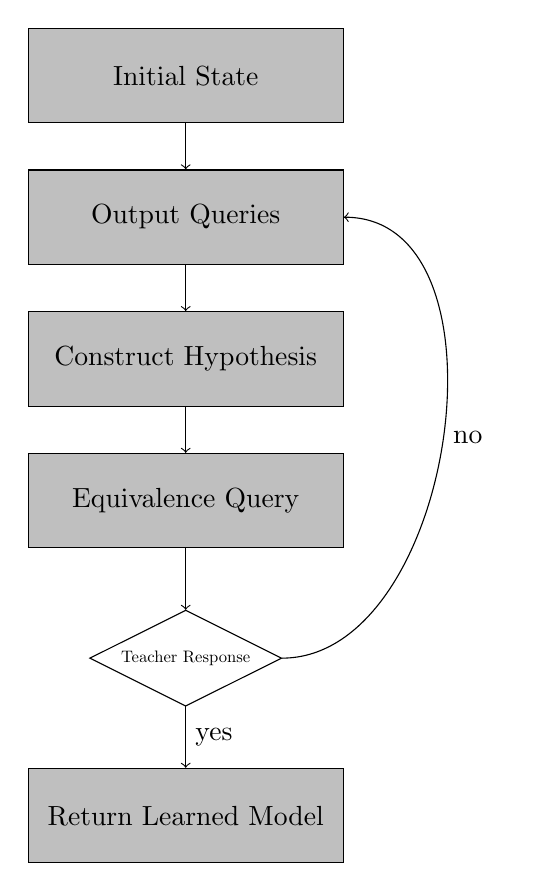
\begin{tikzpicture}[->]
					% Draw the vertices.
					\node at (0,0) [rectangle, draw, fill=lightgray, minimum width=4cm, minimum height=1.2cm] (i) {Initial State};
					\node[rectangle, draw, fill=lightgray, minimum height=1.2cm, below of=i, node distance=1.8cm, minimum width=4cm] (s) {Output Queries};
					\node[rectangle, draw, fill=lightgray, minimum height=1.2cm, below of=s, node distance=1.8cm, minimum width=4cm] (a) {Construct Hypothesis};
					\node[rectangle, draw, below of=a, node distance=1.8cm, fill=lightgray, minimum height=1.2cm, minimum width=4cm] (b) {Equivalence Query};
					\node[diamond, draw, aspect=2, below of=b, node distance=2cm, scale=0.6] (c) {Teacher Response};
					\node[rectangle, draw, below of=c, node distance=2cm, fill=lightgray, minimum height=1.2cm, minimum width=4cm] (d) {Return Learned Model};
					
					% Connect vertices with edges
					\path (i) edge node {} (s);
					\path (s) edge node {} (a);
					\path (a) edge node {} (b);
					\path (b) edge node {} (c);
					\path (c) edge node [right] {yes} (d);
					\path (c) edge [out=0,in=0,looseness=1] node [right] {no} (s);
				\end{tikzpicture}
			}
		\end{column}
		\pause
		\begin{column}{0.4\textwidth}
			 \begin{itemize}
				\item $L^*$ \tiny (Angluin) \normalsize
				\item $KV$ \tiny (Keans and Vazirani)
			\end{itemize}
		\end{column}
	\end{columns}
\end{frame}

\begin{frame}{IPsec}
	\vspace{-1.5em}
	\centering
	\scalebox{0.55}{
		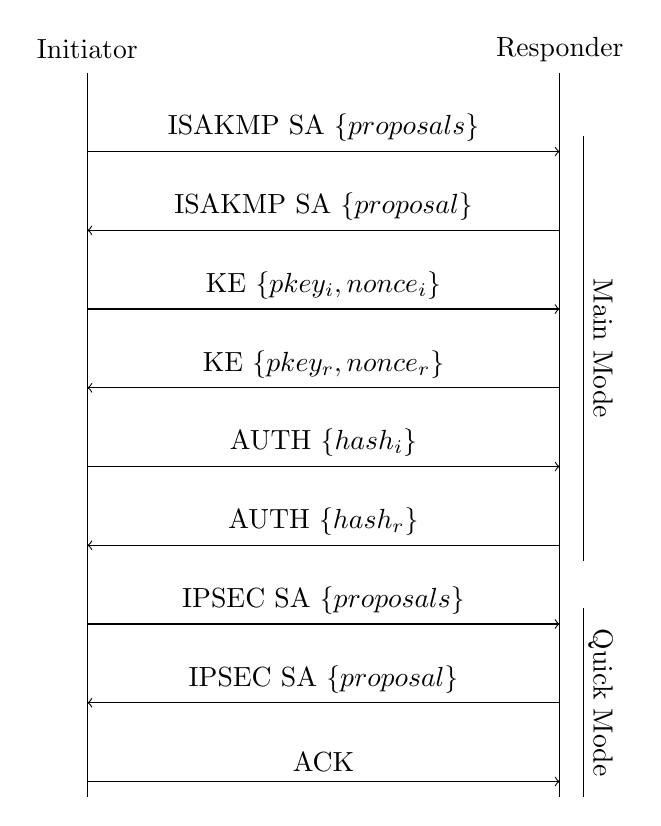
\begin{tikzpicture}
			\draw (-3,0) -- (-3,-9.2) (3,0) -- (3,-9.2);
			\draw (3.3,-0.8) -- node [right=0.9cm, xshift=-0.4cm,rotate=270,anchor=north]  {Main Mode} (3.3,-6.2);
			\draw (3.3,-6.8) -- node [right=0.9cm, xshift=-0.4cm,rotate=270,anchor=north]  {Quick Mode} (3.3,-9.2);
			\node at (-3,.3) {Initiator};
			\node at (3,.3) {Responder};
			\draw[->] (-3,-1) -- node[midway,above] {ISAKMP SA $\{proposals\}$} (3,-1);
			\draw[<-] (-3,-2) -- node[midway,above] {ISAKMP SA $\{proposal\}$} (3,-2);
			\draw[->] (-3,-3) -- node[midway,above] {KE $\{pkey_i, nonce_i\}$} (3,-3);
			\draw[<-] (-3,-4) -- node[midway,above] {KE $\{pkey_r, nonce_r\}$} (3,-4);
			\draw[->] (-3,-5) -- node[midway,above] {AUTH $\{hash_i\}$} (3,-5);
			\draw[<-] (-3,-6) -- node[midway,above] {AUTH $\{hash_r\}$} (3,-6);
			\draw[->] (-3,-7) -- node[midway,above] {IPSEC SA $\{proposals\}$} (3,-7);
			\draw[<-] (-3,-8) -- node[midway,above] {IPSEC SA $\{proposal\}$} (3,-8);
			\draw[->] (-3,-9) -- node[midway,above] {ACK} (3,-9);
		\end{tikzpicture}	
	}
\end{frame}

\begin{frame}{IPsec}
	\vspace{-1.5em}
	\centering
	\scalebox{0.55}{
		\begin{tikzpicture}
			\draw (-3,0) -- (-3,-9.2) (3,0) -- (3,-9.2);
			\draw (3.3,-0.8) -- node [right=0.9cm, xshift=-0.4cm,rotate=270,anchor=north]  {Main Mode} (3.3,-6.2);
			\draw (3.3,-6.8) -- node [right=0.9cm, xshift=-0.4cm,rotate=270,anchor=north]  {Quick Mode} (3.3,-9.2);
			\node at (-3,.3) {Initiator};
			\node at (3,.3) {Responder};
			\draw<1>[red,ultra thick,rounded corners] (-3,-1) rectangle (\textheight-4.5cm,0.05);
			\draw[->] (-3,-1) -- node[midway,above] {ISAKMP SA $\{proposals\}$} (3,-1);
			\draw[<-] (-3,-2) -- node[midway,above] {ISAKMP SA $\{proposal\}$} (3,-2);
			\draw[->] (-3,-3) -- node[midway,above] {KE $\{pkey_i, nonce_i\}$} (3,-3);
			\draw[<-] (-3,-4) -- node[midway,above] {KE $\{pkey_r, nonce_r\}$} (3,-4);
			\draw[->] (-3,-5) -- node[midway,above] {AUTH $\{hash_i\}$} (3,-5);
			\draw[<-] (-3,-6) -- node[midway,above] {AUTH $\{hash_r\}$} (3,-6);
			\draw[->] (-3,-7) -- node[midway,above] {IPSEC SA $\{proposals\}$} (3,-7);
			\draw[<-] (-3,-8) -- node[midway,above] {IPSEC SA $\{proposal\}$} (3,-8);
			\draw[->] (-3,-9) -- node[midway,above] {ACK} (3,-9);
		\end{tikzpicture}	
	}
\end{frame}

\begin{frame}{IPsec}
	\vspace{-1.5em}
	\centering
	\scalebox{0.55}{
		\begin{tikzpicture}
			\draw (-3,0) -- (-3,-9.2) (3,0) -- (3,-9.2);
			\draw (3.3,-0.8) -- node [right=0.9cm, xshift=-0.4cm,rotate=270,anchor=north]  {Main Mode} (3.3,-6.2);
			\draw (3.3,-6.8) -- node [right=0.9cm, xshift=-0.4cm,rotate=270,anchor=north]  {Quick Mode} (3.3,-9.2);
			\node at (-3,.3) {Initiator};
			\node at (3,.3) {Responder};
			\draw[->] (-3,-1) -- node[midway,above] {ISAKMP SA $\{proposals\}$} (3,-1);
			\draw<1>[red,ultra thick,rounded corners] (-3,-2) rectangle (\textheight-4.5cm,-1);
			\draw[<-] (-3,-2) -- node[midway,above] {ISAKMP SA $\{proposal\}$} (3,-2);
			\draw[->] (-3,-3) -- node[midway,above] {KE $\{pkey_i, nonce_i\}$} (3,-3);
			\draw[<-] (-3,-4) -- node[midway,above] {KE $\{pkey_r, nonce_r\}$} (3,-4);
			\draw[->] (-3,-5) -- node[midway,above] {AUTH $\{hash_i\}$} (3,-5);
			\draw[<-] (-3,-6) -- node[midway,above] {AUTH $\{hash_r\}$} (3,-6);
			\draw[->] (-3,-7) -- node[midway,above] {IPSEC SA $\{proposals\}$} (3,-7);
			\draw[<-] (-3,-8) -- node[midway,above] {IPSEC SA $\{proposal\}$} (3,-8);
			\draw[->] (-3,-9) -- node[midway,above] {ACK} (3,-9);
		\end{tikzpicture}	
	}
\end{frame}

\begin{frame}{IPsec}
	\vspace{-1.5em}
	\centering
	\scalebox{0.55}{
		\begin{tikzpicture}
			\draw (-3,0) -- (-3,-9.2) (3,0) -- (3,-9.2);
			\draw (3.3,-0.8) -- node [right=0.9cm, xshift=-0.4cm,rotate=270,anchor=north]  {Main Mode} (3.3,-6.2);
			\draw (3.3,-6.8) -- node [right=0.9cm, xshift=-0.4cm,rotate=270,anchor=north]  {Quick Mode} (3.3,-9.2);
			\node at (-3,.3) {Initiator};
			\node at (3,.3) {Responder};
			\draw[->] (-3,-1) -- node[midway,above] {ISAKMP SA $\{proposals\}$} (3,-1);
			\draw[<-] (-3,-2) -- node[midway,above] {ISAKMP SA $\{proposal\}$} (3,-2);
			\draw<1>[red,ultra thick,rounded corners] (-3,-3) rectangle (\textheight-4.5cm,-2);
			\draw[->] (-3,-3) -- node[midway,above] {KE $\{pkey_i, nonce_i\}$} (3,-3);
			\draw[<-] (-3,-4) -- node[midway,above] {KE $\{pkey_r, nonce_r\}$} (3,-4);
			\draw[->] (-3,-5) -- node[midway,above] {AUTH $\{hash_i\}$} (3,-5);
			\draw[<-] (-3,-6) -- node[midway,above] {AUTH $\{hash_r\}$} (3,-6);
			\draw[->] (-3,-7) -- node[midway,above] {IPSEC SA $\{proposals\}$} (3,-7);
			\draw[<-] (-3,-8) -- node[midway,above] {IPSEC SA $\{proposal\}$} (3,-8);
			\draw[->] (-3,-9) -- node[midway,above] {ACK} (3,-9);
		\end{tikzpicture}	
	}
\end{frame}

\begin{frame}{IPsec}
	\vspace{-1.5em}
	\centering
	\scalebox{0.55}{
		\begin{tikzpicture}
			\draw (-3,0) -- (-3,-9.2) (3,0) -- (3,-9.2);
			\draw (3.3,-0.8) -- node [right=0.9cm, xshift=-0.4cm,rotate=270,anchor=north]  {Main Mode} (3.3,-6.2);
			\draw (3.3,-6.8) -- node [right=0.9cm, xshift=-0.4cm,rotate=270,anchor=north]  {Quick Mode} (3.3,-9.2);
			\node at (-3,.3) {Initiator};
			\node at (3,.3) {Responder};
			\draw[->] (-3,-1) -- node[midway,above] {ISAKMP SA $\{proposals\}$} (3,-1);
			\draw[<-] (-3,-2) -- node[midway,above] {ISAKMP SA $\{proposal\}$} (3,-2);
			\draw[->] (-3,-3) -- node[midway,above] {KE $\{pkey_i, nonce_i\}$} (3,-3);
			\draw<1>[red,ultra thick,rounded corners] (-3,-4) rectangle (\textheight-4.5cm,-3);
			\draw[<-] (-3,-4) -- node[midway,above] {KE $\{pkey_r, nonce_r\}$} (3,-4);
			\draw[->] (-3,-5) -- node[midway,above] {AUTH $\{hash_i\}$} (3,-5);
			\draw[<-] (-3,-6) -- node[midway,above] {AUTH $\{hash_r\}$} (3,-6);
			\draw[->] (-3,-7) -- node[midway,above] {IPSEC SA $\{proposals\}$} (3,-7);
			\draw[<-] (-3,-8) -- node[midway,above] {IPSEC SA $\{proposal\}$} (3,-8);
			\draw[->] (-3,-9) -- node[midway,above] {ACK} (3,-9);
		\end{tikzpicture}	
	}
\end{frame}

\begin{frame}{IPsec}
	\vspace{-1.5em}
	\centering
	\scalebox{0.55}{
		\begin{tikzpicture}
			\draw (-3,0) -- (-3,-9.2) (3,0) -- (3,-9.2);
			\draw (3.3,-0.8) -- node [right=0.9cm, xshift=-0.4cm,rotate=270,anchor=north]  {Main Mode} (3.3,-6.2);
			\draw (3.3,-6.8) -- node [right=0.9cm, xshift=-0.4cm,rotate=270,anchor=north]  {Quick Mode} (3.3,-9.2);
			\node at (-3,.3) {Initiator};
			\node at (3,.3) {Responder};
			\draw[->] (-3,-1) -- node[midway,above] {ISAKMP SA $\{proposals\}$} (3,-1);
			\draw[<-] (-3,-2) -- node[midway,above] {ISAKMP SA $\{proposal\}$} (3,-2);
			\draw[->] (-3,-3) -- node[midway,above] {KE $\{pkey_i, nonce_i\}$} (3,-3);
			\draw[<-] (-3,-4) -- node[midway,above] {KE $\{pkey_r, nonce_r\}$} (3,-4);
			\draw<1>[red,ultra thick,rounded corners] (-3,-5) rectangle (\textheight-4.5cm,-4);
			\draw[->] (-3,-5) -- node[midway,above] {AUTH $\{hash_i\}$} (3,-5);
			\draw[<-] (-3,-6) -- node[midway,above] {AUTH $\{hash_r\}$} (3,-6);
			\draw[->] (-3,-7) -- node[midway,above] {IPSEC SA $\{proposals\}$} (3,-7);
			\draw[<-] (-3,-8) -- node[midway,above] {IPSEC SA $\{proposal\}$} (3,-8);
			\draw[->] (-3,-9) -- node[midway,above] {ACK} (3,-9);
		\end{tikzpicture}	
	}
\end{frame}

\begin{frame}{IPsec}
	\vspace{-1.5em}
	\centering
	\scalebox{0.55}{
		\begin{tikzpicture}
			\draw (-3,0) -- (-3,-9.2) (3,0) -- (3,-9.2);
			\draw (3.3,-0.8) -- node [right=0.9cm, xshift=-0.4cm,rotate=270,anchor=north]  {Main Mode} (3.3,-6.2);
			\draw (3.3,-6.8) -- node [right=0.9cm, xshift=-0.4cm,rotate=270,anchor=north]  {Quick Mode} (3.3,-9.2);
			\node at (-3,.3) {Initiator};
			\node at (3,.3) {Responder};
			\draw[->] (-3,-1) -- node[midway,above] {ISAKMP SA $\{proposals\}$} (3,-1);
			\draw[<-] (-3,-2) -- node[midway,above] {ISAKMP SA $\{proposal\}$} (3,-2);
			\draw[->] (-3,-3) -- node[midway,above] {KE $\{pkey_i, nonce_i\}$} (3,-3);
			\draw[<-] (-3,-4) -- node[midway,above] {KE $\{pkey_r, nonce_r\}$} (3,-4);
			\draw[->] (-3,-5) -- node[midway,above] {AUTH $\{hash_i\}$} (3,-5);
			\draw<1>[red,ultra thick,rounded corners] (-3,-6) rectangle (\textheight-4.5cm,-5);
			\draw[<-] (-3,-6) -- node[midway,above] {AUTH $\{hash_r\}$} (3,-6);
			\draw[->] (-3,-7) -- node[midway,above] {IPSEC SA $\{proposals\}$} (3,-7);
			\draw[<-] (-3,-8) -- node[midway,above] {IPSEC SA $\{proposal\}$} (3,-8);
			\draw[->] (-3,-9) -- node[midway,above] {ACK} (3,-9);
		\end{tikzpicture}	
	}
\end{frame}

\begin{frame}{IPsec}
	\vspace{-1.5em}
	\centering
	\scalebox{0.55}{
		\begin{tikzpicture}
			\draw (-3,0) -- (-3,-9.2) (3,0) -- (3,-9.2);
			\draw (3.3,-0.8) -- node [right=0.9cm, xshift=-0.4cm,rotate=270,anchor=north]  {Main Mode} (3.3,-6.2);
			\draw (3.3,-6.8) -- node [right=0.9cm, xshift=-0.4cm,rotate=270,anchor=north]  {Quick Mode} (3.3,-9.2);
			\node at (-3,.3) {Initiator};
			\node at (3,.3) {Responder};
			\draw[->] (-3,-1) -- node[midway,above] {ISAKMP SA $\{proposals\}$} (3,-1);
			\draw[<-] (-3,-2) -- node[midway,above] {ISAKMP SA $\{proposal\}$} (3,-2);
			\draw[->] (-3,-3) -- node[midway,above] {KE $\{pkey_i, nonce_i\}$} (3,-3);
			\draw[<-] (-3,-4) -- node[midway,above] {KE $\{pkey_r, nonce_r\}$} (3,-4);
			\draw[->] (-3,-5) -- node[midway,above] {AUTH $\{hash_i\}$} (3,-5);
			\draw[<-] (-3,-6) -- node[midway,above] {AUTH $\{hash_r\}$} (3,-6);
			\draw<1>[red,ultra thick,rounded corners] (-3,-7) rectangle (\textheight-4.5cm,-6);
			\draw[->] (-3,-7) -- node[midway,above] {IPSEC SA $\{proposals\}$} (3,-7);
			\draw[<-] (-3,-8) -- node[midway,above] {IPSEC SA $\{proposal\}$} (3,-8);
			\draw[->] (-3,-9) -- node[midway,above] {ACK} (3,-9);
		\end{tikzpicture}	
	}
\end{frame}

\begin{frame}{IPsec}
	\vspace{-1.5em}
	\centering
	\scalebox{0.55}{
		\begin{tikzpicture}
			\draw (-3,0) -- (-3,-9.2) (3,0) -- (3,-9.2);
			\draw (3.3,-0.8) -- node [right=0.9cm, xshift=-0.4cm,rotate=270,anchor=north]  {Main Mode} (3.3,-6.2);
			\draw (3.3,-6.8) -- node [right=0.9cm, xshift=-0.4cm,rotate=270,anchor=north]  {Quick Mode} (3.3,-9.2);
			\node at (-3,.3) {Initiator};
			\node at (3,.3) {Responder};
			\draw[->] (-3,-1) -- node[midway,above] {ISAKMP SA $\{proposals\}$} (3,-1);
			\draw[<-] (-3,-2) -- node[midway,above] {ISAKMP SA $\{proposal\}$} (3,-2);
			\draw[->] (-3,-3) -- node[midway,above] {KE $\{pkey_i, nonce_i\}$} (3,-3);
			\draw[<-] (-3,-4) -- node[midway,above] {KE $\{pkey_r, nonce_r\}$} (3,-4);
			\draw[->] (-3,-5) -- node[midway,above] {AUTH $\{hash_i\}$} (3,-5);
			\draw[<-] (-3,-6) -- node[midway,above] {AUTH $\{hash_r\}$} (3,-6);
			\draw[->] (-3,-7) -- node[midway,above] {IPSEC SA $\{proposals\}$} (3,-7);
			\draw<1>[red,ultra thick,rounded corners] (-3,-8) rectangle (\textheight-4.5cm,-7);
			\draw[<-] (-3,-8) -- node[midway,above] {IPSEC SA $\{proposal\}$} (3,-8);
			\draw[->] (-3,-9) -- node[midway,above] {ACK} (3,-9);
		\end{tikzpicture}	
	}
\end{frame}

\begin{frame}{IPsec}
	\vspace{-1.5em}
	\centering
	\scalebox{0.55}{
		\begin{tikzpicture}
			\draw (-3,0) -- (-3,-9.2) (3,0) -- (3,-9.2);
			\draw (3.3,-0.8) -- node [right=0.9cm, xshift=-0.4cm,rotate=270,anchor=north]  {Main Mode} (3.3,-6.2);
			\draw (3.3,-6.8) -- node [right=0.9cm, xshift=-0.4cm,rotate=270,anchor=north]  {Quick Mode} (3.3,-9.2);
			\node at (-3,.3) {Initiator};
			\node at (3,.3) {Responder};
			\draw[->] (-3,-1) -- node[midway,above] {ISAKMP SA $\{proposals\}$} (3,-1);
			\draw[<-] (-3,-2) -- node[midway,above] {ISAKMP SA $\{proposal\}$} (3,-2);
			\draw[->] (-3,-3) -- node[midway,above] {KE $\{pkey_i, nonce_i\}$} (3,-3);
			\draw[<-] (-3,-4) -- node[midway,above] {KE $\{pkey_r, nonce_r\}$} (3,-4);
			\draw[->] (-3,-5) -- node[midway,above] {AUTH $\{hash_i\}$} (3,-5);
			\draw[<-] (-3,-6) -- node[midway,above] {AUTH $\{hash_r\}$} (3,-6);
			\draw[->] (-3,-7) -- node[midway,above] {IPSEC SA $\{proposals\}$} (3,-7);
			\draw[<-] (-3,-8) -- node[midway,above] {IPSEC SA $\{proposal\}$} (3,-8);
			\draw<1>[red,ultra thick,rounded corners] (-3,-9) rectangle (\textheight-4.5cm,-8);
			\draw[->] (-3,-9) -- node[midway,above] {ACK} (3,-9);
		\end{tikzpicture}	
	}
\end{frame}
%maybe fuzzing?
% maybe other order: IPsec -> learning -> fuzzing

\section{Model Learning}

\begin{frame}{Environment Setup}
  \vspace{-1.5em}
  \begin{itemize}
  	\item Ubuntu 22.04 LTS VM pairs
  	\pause
  	\item Dedicated virtualized network
  	\pause
  	\item Responder (SUL) / Initiator (learner)
  	\pause
  	\item strongSwan \& libreswan SUL
  \end{itemize}
\end{frame}


%- reiterate on how the learning works by repeatedly querying the SUL
%- highlight mapper class as our biggest achievement
\begin{frame}{Learning Pipeline}
	\scalebox{0.8}{
		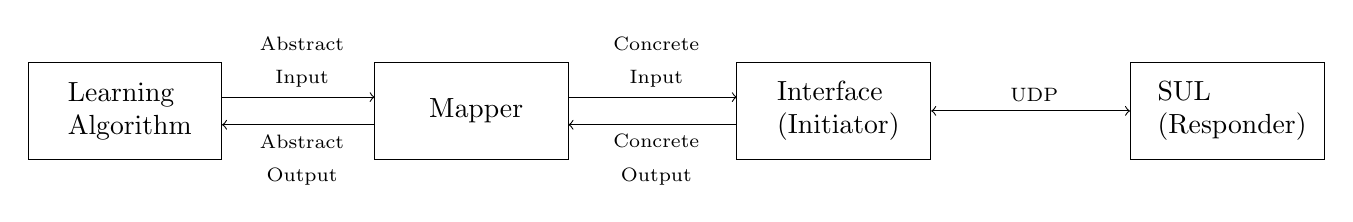
\begin{tikzpicture} 
			\node (n1) [draw, minimum width=7em, minimum height=3.5em, align=left] at (0,1) {~Learning\\~Algorithm};
			\node (n2) [draw, minimum width=7em, minimum height=3.5em, align=left] at (4.4,1) {~Mapper};
			\node(n3) [draw, minimum width=7em, minimum height=3.5em,  align=left] at (9,1) {~Interface\\~(Initiator)};
			\node(n4) [draw, minimum width=7em, minimum height=3.5em,  align=left] at (14,1) {~SUL\\~(Responder)};
			\draw [->] ($(n1)+(3.5em,+0.5em)$) -> ($(n2)+(-3.5em,+0.5em)$) node[midway,above,align=center] {\scriptsize~Abstract\\\scriptsize~Input};
			\draw [->] ($(n2)+(-3.5em,-0.5em)$) -> ($(n1)+(3.5em,-0.5em)$) node[midway,below,align=center] {\scriptsize~Abstract\\\scriptsize~Output};
			
			\draw [->] ($(n2)+(3.5em,+0.5em)$) -> ($(n3)+(-3.5em,+0.5em)$) node[midway,above,align=center] {\scriptsize~Concrete\\\scriptsize~Input};
			\draw [->] ($(n3)+(-3.5em,-0.5em)$) -> ($(n2)+(3.5em,-0.5em)$) node[midway,below,align=center] {\scriptsize~Concrete\\\scriptsize~Output};
			
			\draw [<->] (n3) -> (n4) node[midway,above,align=center] {\scriptsize~UDP};
		\end{tikzpicture} 
	}
\end{frame}

\begin{frame}{Learning Pipeline}
	\scalebox{0.8}{
		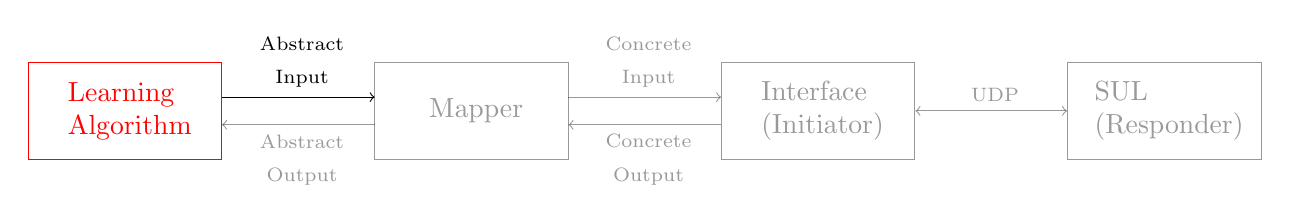
\begin{tikzpicture} 
			\node (n1) [draw, minimum width=7em, minimum height=3.5em, align=left, color=red] at (0,1) {~Learning\\~Algorithm};
			\node (n2) [draw, minimum width=7em, minimum height=3.5em, align=left, opacity=0.4] at (4.4,1) {~Mapper};
			\node(n3) [draw, minimum width=7em, minimum height=3.5em,  align=left, opacity=0.4] at (8.8,1) {~Interface\\~(Initiator)};
			\node(n4) [draw, minimum width=7em, minimum height=3.5em,  align=left, opacity=0.4] at (13.2,1) {~SUL\\~(Responder)};
			\draw [->] ($(n1)+(3.5em,+0.5em)$) -> ($(n2)+(-3.5em,+0.5em)$) node[midway,above,align=center] {\scriptsize~Abstract\\\scriptsize~Input};
			\draw [->, opacity=0.4] ($(n2)+(-3.5em,-0.5em)$) -> ($(n1)+(3.5em,-0.5em)$) node[midway,below,align=center, opacity=0.4] {\scriptsize~Abstract\\\scriptsize~Output};
			
			\draw [->, opacity=0.4] ($(n2)+(3.5em,+0.5em)$) -> ($(n3)+(-3.5em,+0.5em)$) node[midway,above,align=center, opacity=0.4] {\scriptsize~Concrete\\\scriptsize~Input};
			\draw [->, opacity=0.4] ($(n3)+(-3.5em,-0.5em)$) -> ($(n2)+(3.5em,-0.5em)$) node[midway,below,align=center, opacity=0.4] {\scriptsize~Concrete\\\scriptsize~Output};
			
			\draw [<->, opacity=0.4] (n3) -> (n4) node[midway,above,align=center, opacity=0.4] {\scriptsize~UDP};
		\end{tikzpicture} 
	}
	\begin{itemize}
		\item AALpy
		\item $KV$ / $L^{*}$
	\end{itemize}
\end{frame}

\begin{frame}{Learning Pipeline}
	\scalebox{0.8}{
		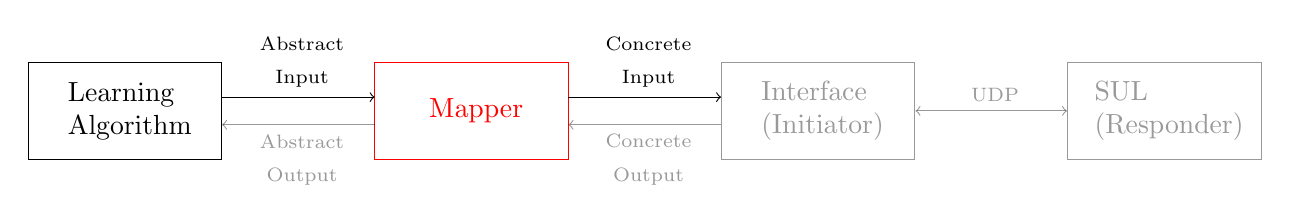
\begin{tikzpicture} 
			\node (n1) [draw, minimum width=7em, minimum height=3.5em, align=left] at (0,1) {~Learning\\~Algorithm};
			\node (n2) [draw, minimum width=7em, minimum height=3.5em, align=left, color=red] at (4.4,1) {~Mapper};
			\node(n3) [draw, minimum width=7em, minimum height=3.5em,  align=left, opacity=0.4] at (8.8,1) {~Interface\\~(Initiator)};
			\node(n4) [draw, minimum width=7em, minimum height=3.5em,  align=left, opacity=0.4] at (13.2,1) {~SUL\\~(Responder)};
			\draw [->] ($(n1)+(3.5em,+0.5em)$) -> ($(n2)+(-3.5em,+0.5em)$) node[midway,above,align=center] {\scriptsize~Abstract\\\scriptsize~Input};
			\draw [->, opacity=0.4] ($(n2)+(-3.5em,-0.5em)$) -> ($(n1)+(3.5em,-0.5em)$) node[midway,below,align=center, opacity=0.4] {\scriptsize~Abstract\\\scriptsize~Output};
			
			\draw [->] ($(n2)+(3.5em,+0.5em)$) -> ($(n3)+(-3.5em,+0.5em)$) node[midway,above,align=center] {\scriptsize~Concrete\\\scriptsize~Input};
			\draw [->, opacity=0.4] ($(n3)+(-3.5em,-0.5em)$) -> ($(n2)+(3.5em,-0.5em)$) node[midway,below,align=center, opacity=0.4] {\scriptsize~Concrete\\\scriptsize~Output};
			
			\draw [<->, opacity=0.4] (n3) -> (n4) node[midway,above,align=center, opacity=0.4] {\scriptsize~UDP};
		\end{tikzpicture} 
	}
	\begin{itemize}
		\item Scapy %modular
		\item Key management
		\item Error and retransmission handling
	\end{itemize}
\end{frame}

\begin{frame}{Learning Pipeline}
	\scalebox{0.8}{
		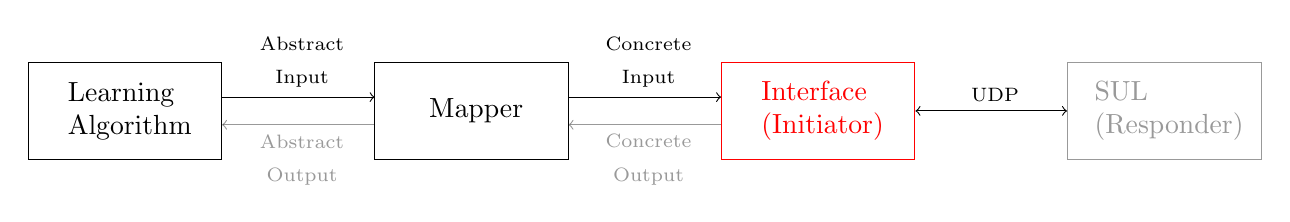
\begin{tikzpicture} 
			\node (n1) [draw, minimum width=7em, minimum height=3.5em, align=left] at (0,1) {~Learning\\~Algorithm};
			\node (n2) [draw, minimum width=7em, minimum height=3.5em, align=left] at (4.4,1) {~Mapper};
			\node(n3) [draw, minimum width=7em, minimum height=3.5em,  align=left, color=red] at (8.8,1) {~Interface\\~(Initiator)};
			\node(n4) [draw, minimum width=7em, minimum height=3.5em,  align=left, opacity=0.4] at (13.2,1) {~SUL\\~(Responder)};
			\draw [->] ($(n1)+(3.5em,+0.5em)$) -> ($(n2)+(-3.5em,+0.5em)$) node[midway,above,align=center] {\scriptsize~Abstract\\\scriptsize~Input};
			\draw [->, opacity=0.4] ($(n2)+(-3.5em,-0.5em)$) -> ($(n1)+(3.5em,-0.5em)$) node[midway,below,align=center, opacity=0.4] {\scriptsize~Abstract\\\scriptsize~Output};
			
			\draw [->] ($(n2)+(3.5em,+0.5em)$) -> ($(n3)+(-3.5em,+0.5em)$) node[midway,above,align=center] {\scriptsize~Concrete\\\scriptsize~Input};
			\draw [->, opacity=0.4] ($(n3)+(-3.5em,-0.5em)$) -> ($(n2)+(3.5em,-0.5em)$) node[midway,below,align=center, opacity=0.4] {\scriptsize~Concrete\\\scriptsize~Output};
			
			\draw [<->] (n3) -> (n4) node[midway,above,align=center] {\scriptsize~UDP};
		\end{tikzpicture} 
	}
	\begin{itemize}
		\item Simple UDP socket wrapper
		\item Works with Scapy packets % don't use scapy send method directly to add encapsulation, and the possibility of easily sending malformed packets for fuzzing. Also we have a workaround for libreswan with the manual resets
	\end{itemize}
\end{frame}

\begin{frame}{Learning Pipeline}
	\scalebox{0.8}{
		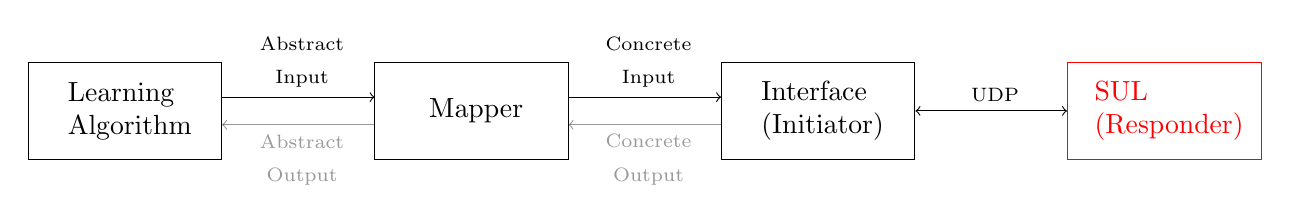
\begin{tikzpicture} 
			\node (n1) [draw, minimum width=7em, minimum height=3.5em, align=left] at (0,1) {~Learning\\~Algorithm};
			\node (n2) [draw, minimum width=7em, minimum height=3.5em, align=left] at (4.4,1) {~Mapper};
			\node(n3) [draw, minimum width=7em, minimum height=3.5em,  align=left] at (8.8,1) {~Interface\\~(Initiator)};
			\node(n4) [draw, minimum width=7em, minimum height=3.5em,  align=left, color=red] at (13.2,1) {~SUL\\~(Responder)};
			\draw [->] ($(n1)+(3.5em,+0.5em)$) -> ($(n2)+(-3.5em,+0.5em)$) node[midway,above,align=center] {\scriptsize~Abstract\\\scriptsize~Input};
			\draw [->, opacity=0.4] ($(n2)+(-3.5em,-0.5em)$) -> ($(n1)+(3.5em,-0.5em)$) node[midway,below,align=center, opacity=0.4] {\scriptsize~Abstract\\\scriptsize~Output};
			
			\draw [->] ($(n2)+(3.5em,+0.5em)$) -> ($(n3)+(-3.5em,+0.5em)$) node[midway,above,align=center] {\scriptsize~Concrete\\\scriptsize~Input};
			\draw [->, opacity=0.4] ($(n3)+(-3.5em,-0.5em)$) -> ($(n2)+(3.5em,-0.5em)$) node[midway,below,align=center, opacity=0.4] {\scriptsize~Concrete\\\scriptsize~Output};
			
			\draw [<->] (n3) -> (n4) node[midway,above,align=center] {\scriptsize~UDP};
		\end{tikzpicture} 
	}
	\begin{itemize}
		\item SUL parses packet
	\end{itemize}
\end{frame}

\begin{frame}{Learning Pipeline}
	\scalebox{0.8}{
		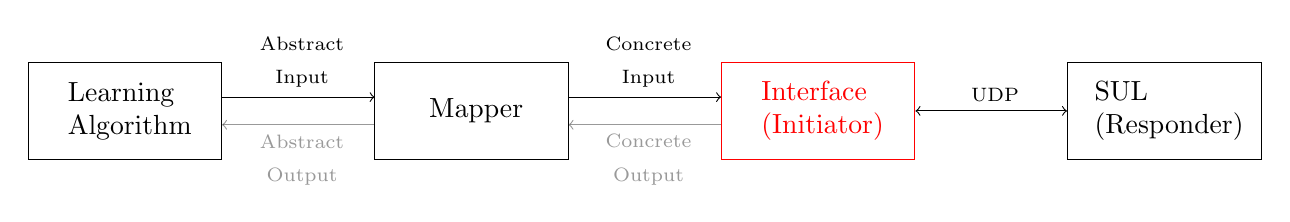
\begin{tikzpicture} 
			\node (n1) [draw, minimum width=7em, minimum height=3.5em, align=left] at (0,1) {~Learning\\~Algorithm};
			\node (n2) [draw, minimum width=7em, minimum height=3.5em, align=left] at (4.4,1) {~Mapper};
			\node(n3) [draw, minimum width=7em, minimum height=3.5em,  align=left, color=red] at (8.8,1) {~Interface\\~(Initiator)};
			\node(n4) [draw, minimum width=7em, minimum height=3.5em,  align=left] at (13.2,1) {~SUL\\~(Responder)};
			\draw [->] ($(n1)+(3.5em,+0.5em)$) -> ($(n2)+(-3.5em,+0.5em)$) node[midway,above,align=center] {\scriptsize~Abstract\\\scriptsize~Input};
			\draw [->, opacity=0.4] ($(n2)+(-3.5em,-0.5em)$) -> ($(n1)+(3.5em,-0.5em)$) node[midway,below,align=center, opacity=0.4] {\scriptsize~Abstract\\\scriptsize~Output};
			
			\draw [->] ($(n2)+(3.5em,+0.5em)$) -> ($(n3)+(-3.5em,+0.5em)$) node[midway,above,align=center] {\scriptsize~Concrete\\\scriptsize~Input};
			\draw [->, opacity=0.4] ($(n3)+(-3.5em,-0.5em)$) -> ($(n2)+(3.5em,-0.5em)$) node[midway,below,align=center] {\scriptsize~Concrete\\\scriptsize~Output};
			
			\draw [<->] (n3) -> (n4) node[midway,above,align=center] {\scriptsize~UDP};
		\end{tikzpicture} 
	}
	\begin{itemize}
		\item Unpack response
		\item Returns Scapy packet
	\end{itemize}
\end{frame}

\begin{frame}{Learning Pipeline}
	\scalebox{0.8}{
		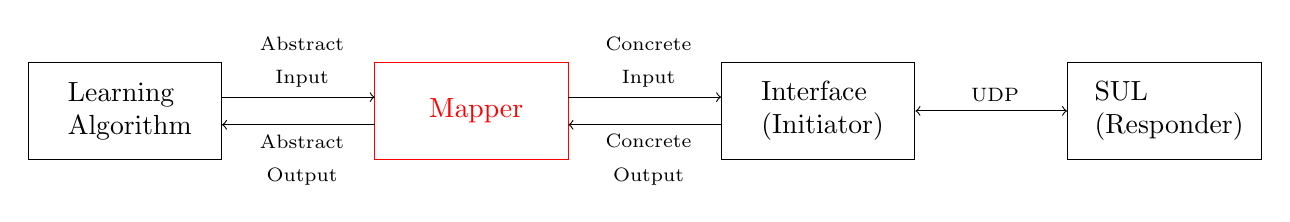
\begin{tikzpicture} 
			\node (n1) [draw, minimum width=7em, minimum height=3.5em, align=left] at (0,1) {~Learning\\~Algorithm};
			\node (n2) [draw, minimum width=7em, minimum height=3.5em, align=left, color=red] at (4.4,1) {~Mapper};
			\node(n3) [draw, minimum width=7em, minimum height=3.5em,  align=left] at (8.8,1) {~Interface\\~(Initiator)};
			\node(n4) [draw, minimum width=7em, minimum height=3.5em,  align=left] at (13.2,1) {~SUL\\~(Responder)};
			\draw [->] ($(n1)+(3.5em,+0.5em)$) -> ($(n2)+(-3.5em,+0.5em)$) node[midway,above,align=center] {\scriptsize~Abstract\\\scriptsize~Input};
			\draw [->] ($(n2)+(-3.5em,-0.5em)$) -> ($(n1)+(3.5em,-0.5em)$) node[midway,below,align=center] {\scriptsize~Abstract\\\scriptsize~Output};
			
			\draw [->] ($(n2)+(3.5em,+0.5em)$) -> ($(n3)+(-3.5em,+0.5em)$) node[midway,above,align=center] {\scriptsize~Concrete\\\scriptsize~Input};
			\draw [->] ($(n3)+(-3.5em,-0.5em)$) -> ($(n2)+(3.5em,-0.5em)$) node[midway,below,align=center] {\scriptsize~Concrete\\\scriptsize~Output};
			
			\draw [<->] (n3) -> (n4) node[midway,above,align=center] {\scriptsize~UDP};
		\end{tikzpicture} 
	}
	\begin{itemize}
		\item Parse packet
		\item Update datastructures
	\end{itemize}
\end{frame}

\begin{frame}{Learning Pipeline}
	\scalebox{0.8}{
		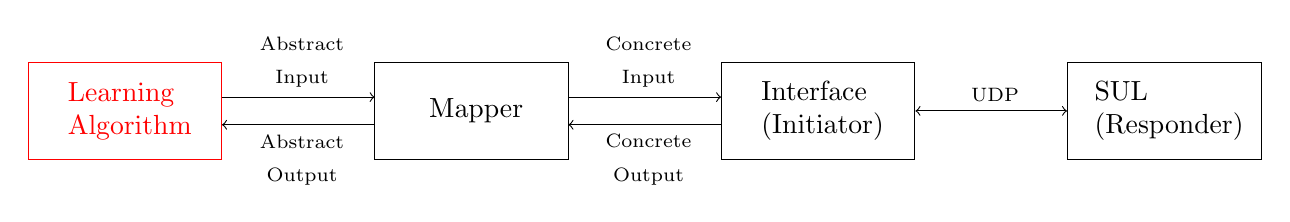
\begin{tikzpicture} 
			\node (n1) [draw, minimum width=7em, minimum height=3.5em, align=left, color=red] at (0,1) {~Learning\\~Algorithm};
			\node (n2) [draw, minimum width=7em, minimum height=3.5em, align=left] at (4.4,1) {~Mapper};
			\node(n3) [draw, minimum width=7em, minimum height=3.5em,  align=left] at (8.8,1) {~Interface\\~(Initiator)};
			\node(n4) [draw, minimum width=7em, minimum height=3.5em,  align=left] at (13.2,1) {~SUL\\~(Responder)};
			\draw [->] ($(n1)+(3.5em,+0.5em)$) -> ($(n2)+(-3.5em,+0.5em)$) node[midway,above,align=center] {\scriptsize~Abstract\\\scriptsize~Input};
			\draw [->] ($(n2)+(-3.5em,-0.5em)$) -> ($(n1)+(3.5em,-0.5em)$) node[midway,below,align=center] {\scriptsize~Abstract\\\scriptsize~Output};
			
			\draw [->] ($(n2)+(3.5em,+0.5em)$) -> ($(n3)+(-3.5em,+0.5em)$) node[midway,above,align=center] {\scriptsize~Concrete\\\scriptsize~Input};
			\draw [->] ($(n3)+(-3.5em,-0.5em)$) -> ($(n2)+(3.5em,-0.5em)$) node[midway,below,align=center] {\scriptsize~Concrete\\\scriptsize~Output};
			
			\draw [<->] (n3) -> (n4) node[midway,above,align=center] {\scriptsize~UDP};
		\end{tikzpicture} 
	}
\end{frame}

\begin{frame}{Challenges}
	\vspace{-1.5em}
	\begin{columns}[T]
		\begin{column}{0.5\textwidth}
			\begin{itemize}
				\item Handling state % mention we look at only the most recet TODO: check that this is true!
				\pause
				\item Timing problems % tuning timeouts to achieve consistent results in reasonable time
				\pause
				\item Retransmissions
				\pause
				\item Difficult debugging
				\pause
				\item Library error % after all the previously mentioned fixes, still had frequent, yet random errors
				\pause
				\item Resource limitations % anecdotally mention motherboard dieing on me, luckily still under warrenty
			\end{itemize}
		\end{column}
		\begin{column}{0.5\textwidth}
			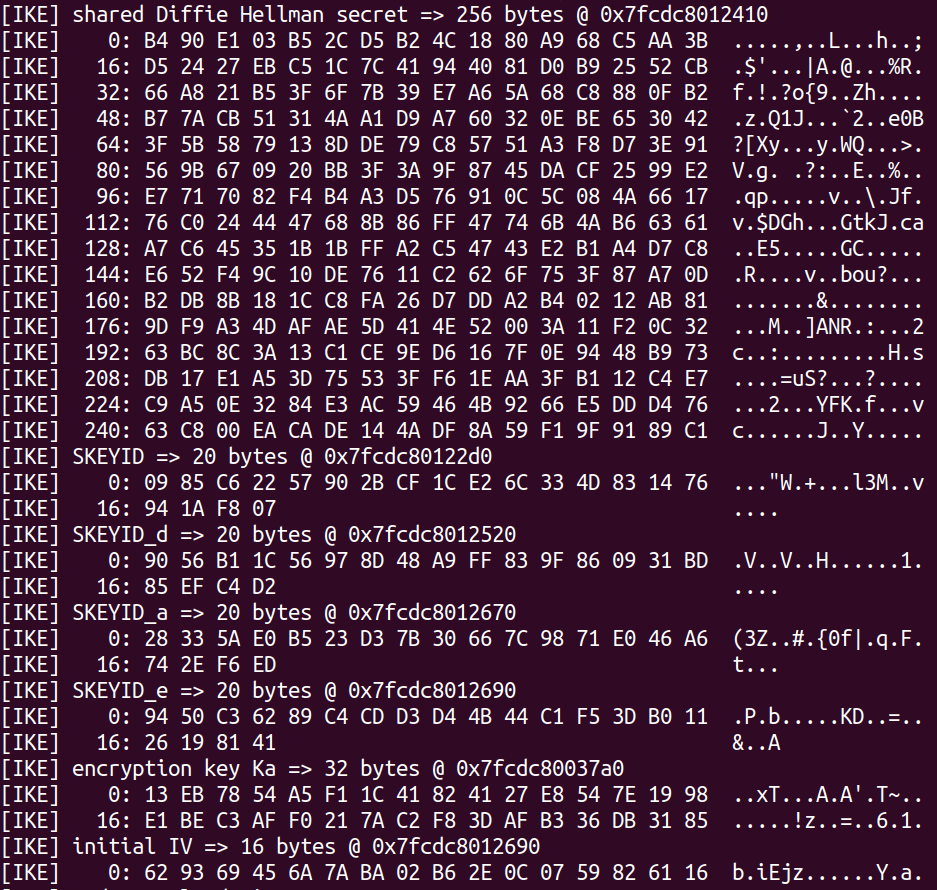
\includegraphics[width=0.85\linewidth]{images/key_material_log}
		\end{column}
	\end{columns}
\end{frame}

\section*{Learned Models}

\begin{frame}{Model Overview}
	%Highlight the various models and how / why they were learned
	\vspace{-1.5em}
	\begin{itemize}
		\item StrongSwan Base
		\item StrongSwan Fuzzing Reference
		\pause
		\item libreswan Base
		\item libreswan Fuzzing Reference
		%\pause
		%\item Retransmission Sample 1
		%\item Retransmission Sample 2
	\end{itemize}
\end{frame}

\begin{frame}{StrongSwan Base}
	\vspace{-4em}
	\centering
	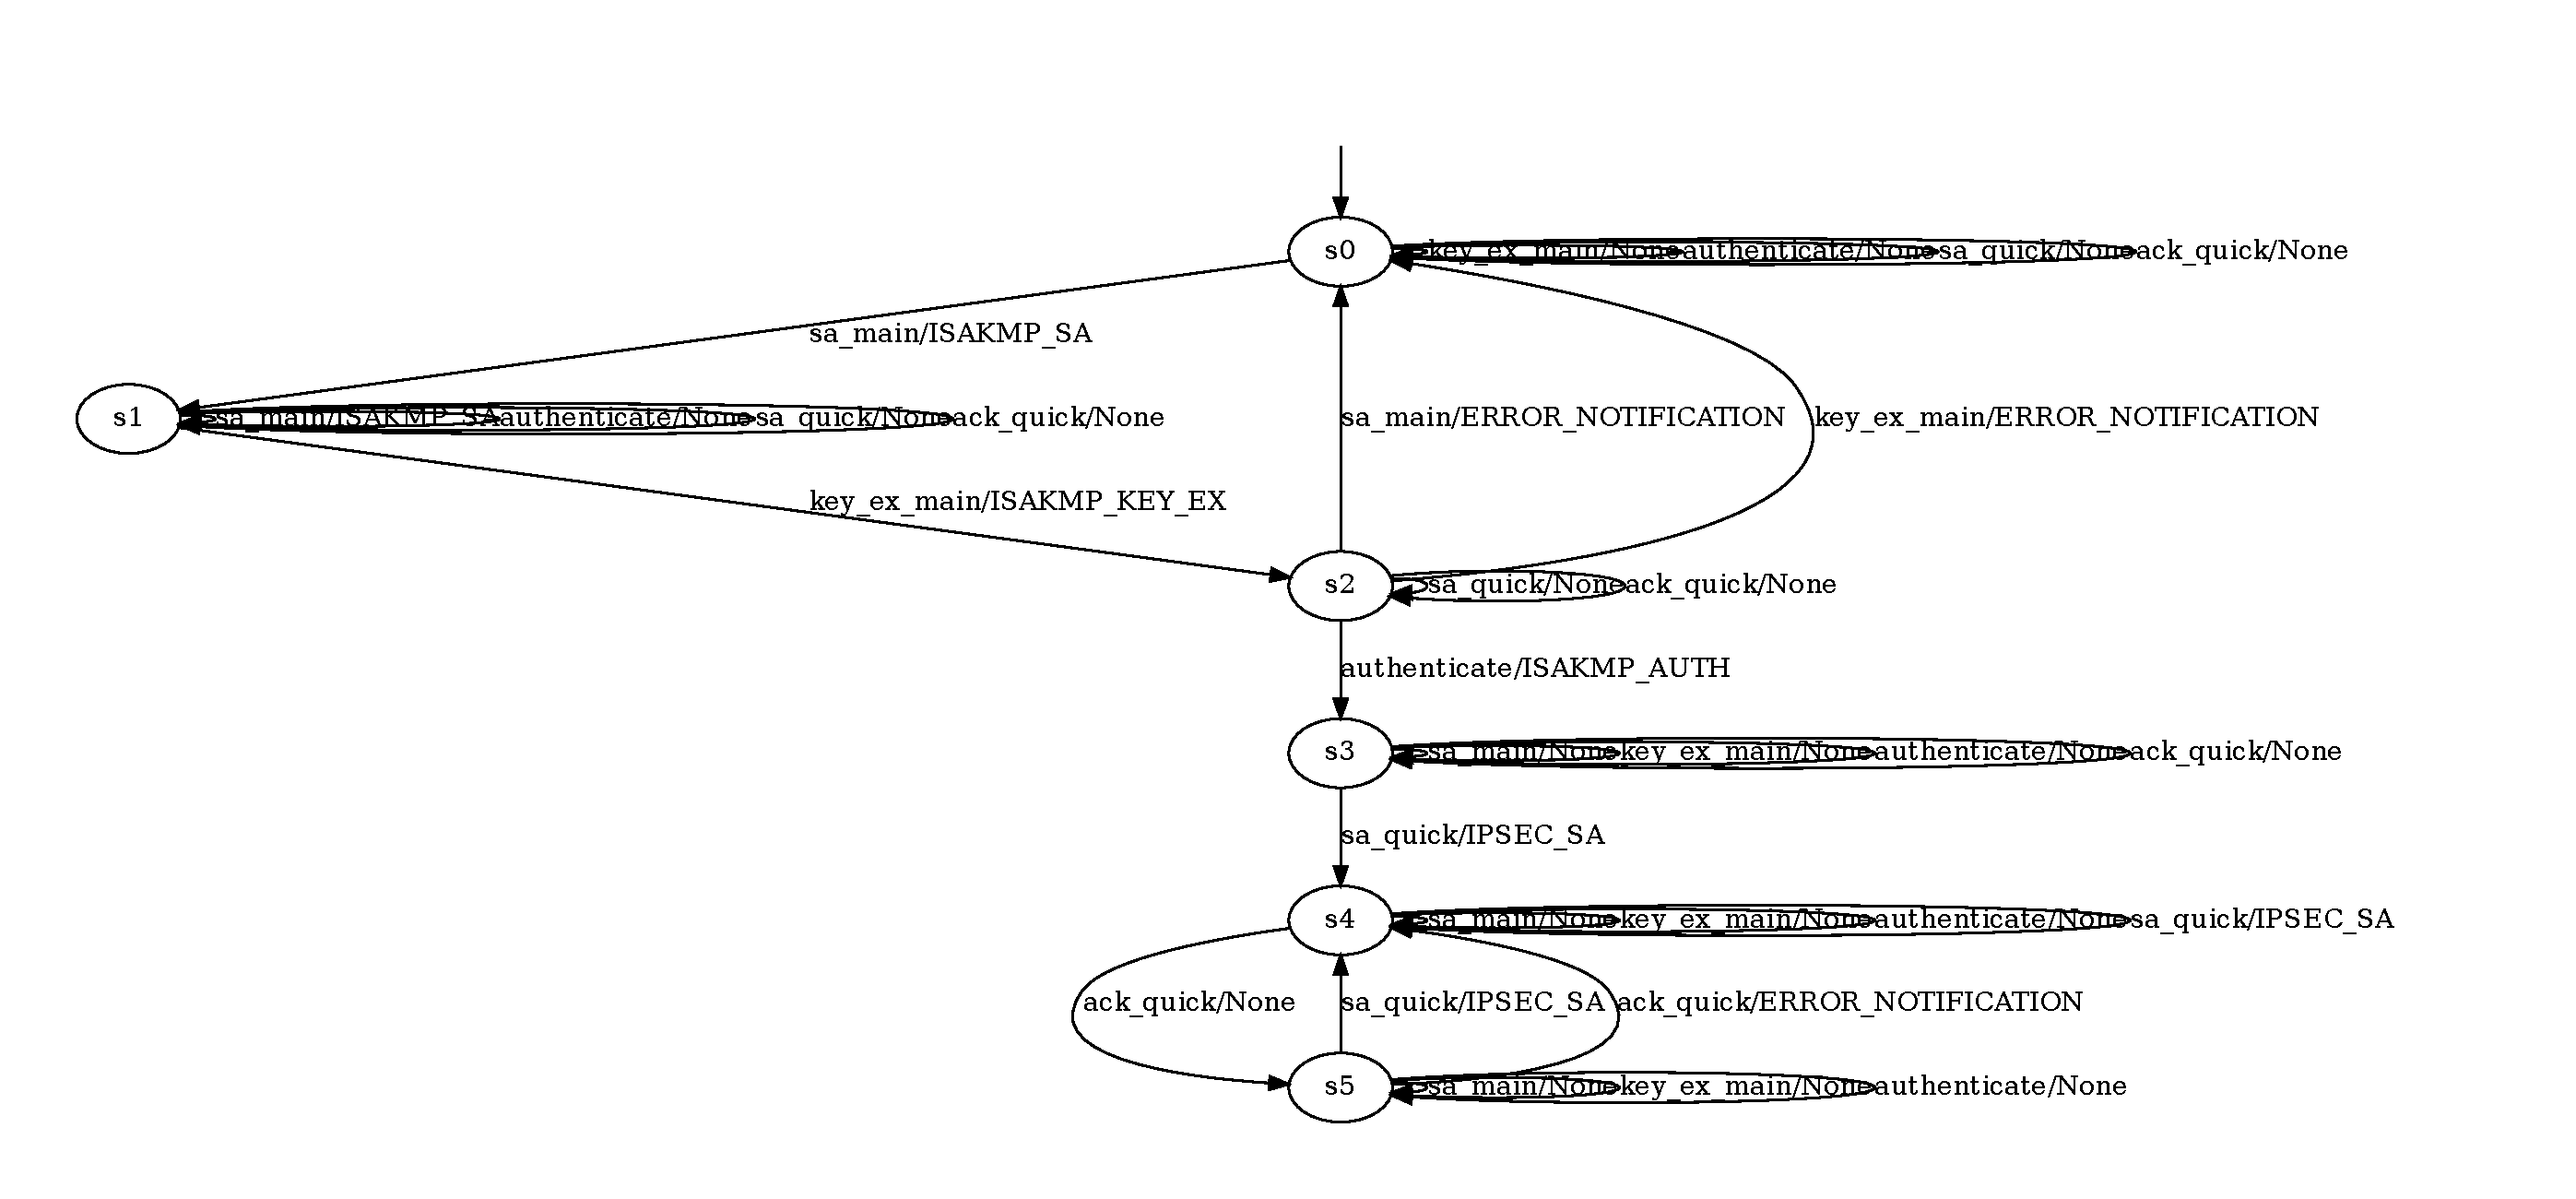
\includegraphics[height=0.9\textheight, trim={8em 0 0 0}]{models/Reference.pdf}
\end{frame}

\begin{frame}{StrongSwan Fuzzing Reference (Simplified)}
	\vspace{-4em}
	\centering
	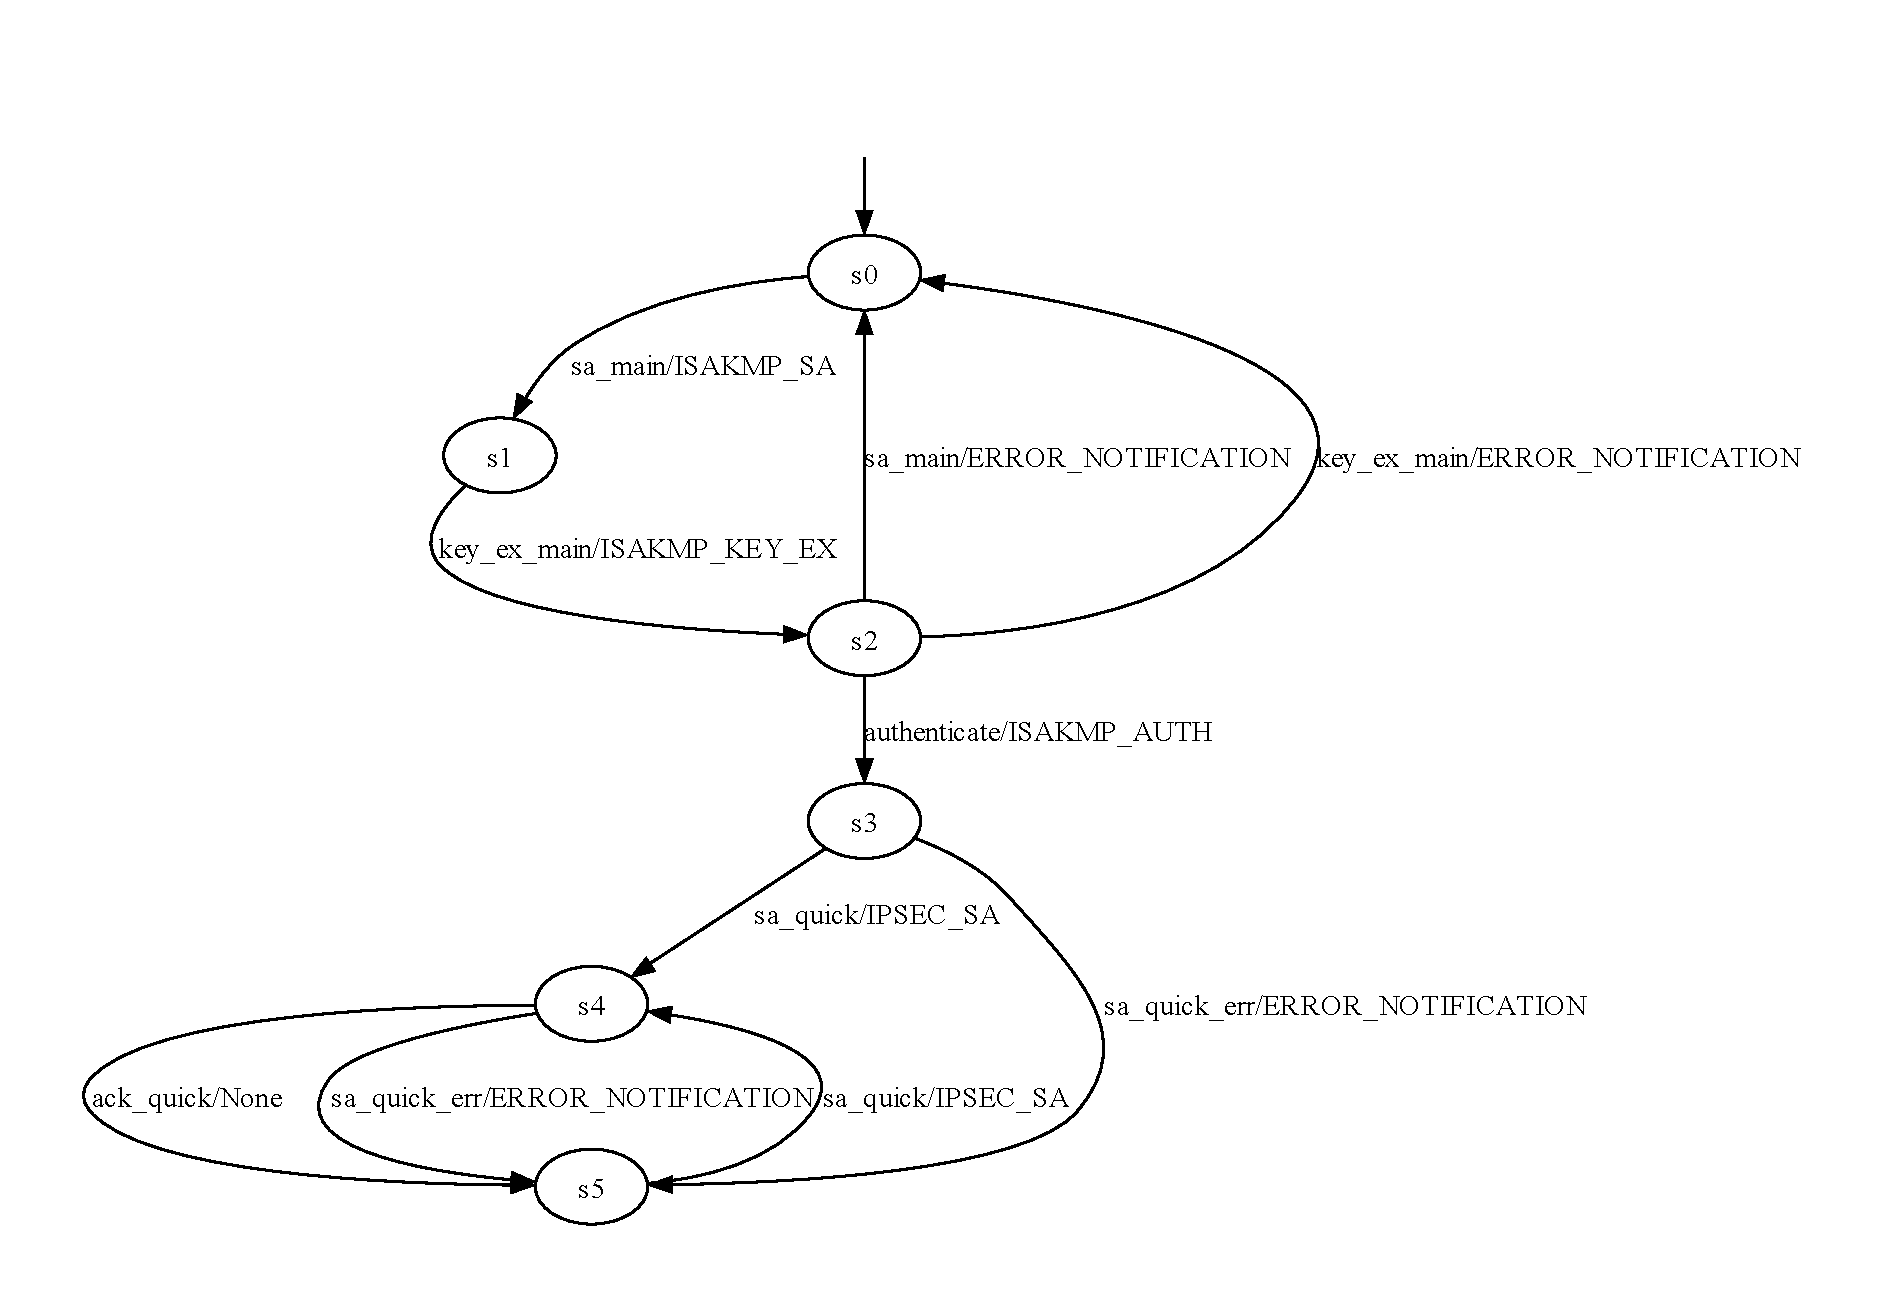
\includegraphics[height=1.0\textheight, trim={8em 0 0 0}]{models/strongSwanErrKV.pdf}
\end{frame}

%TODO maybe redo more readably
\begin{frame}{libreswan Base}
	\vspace{-3em}
	\centering
	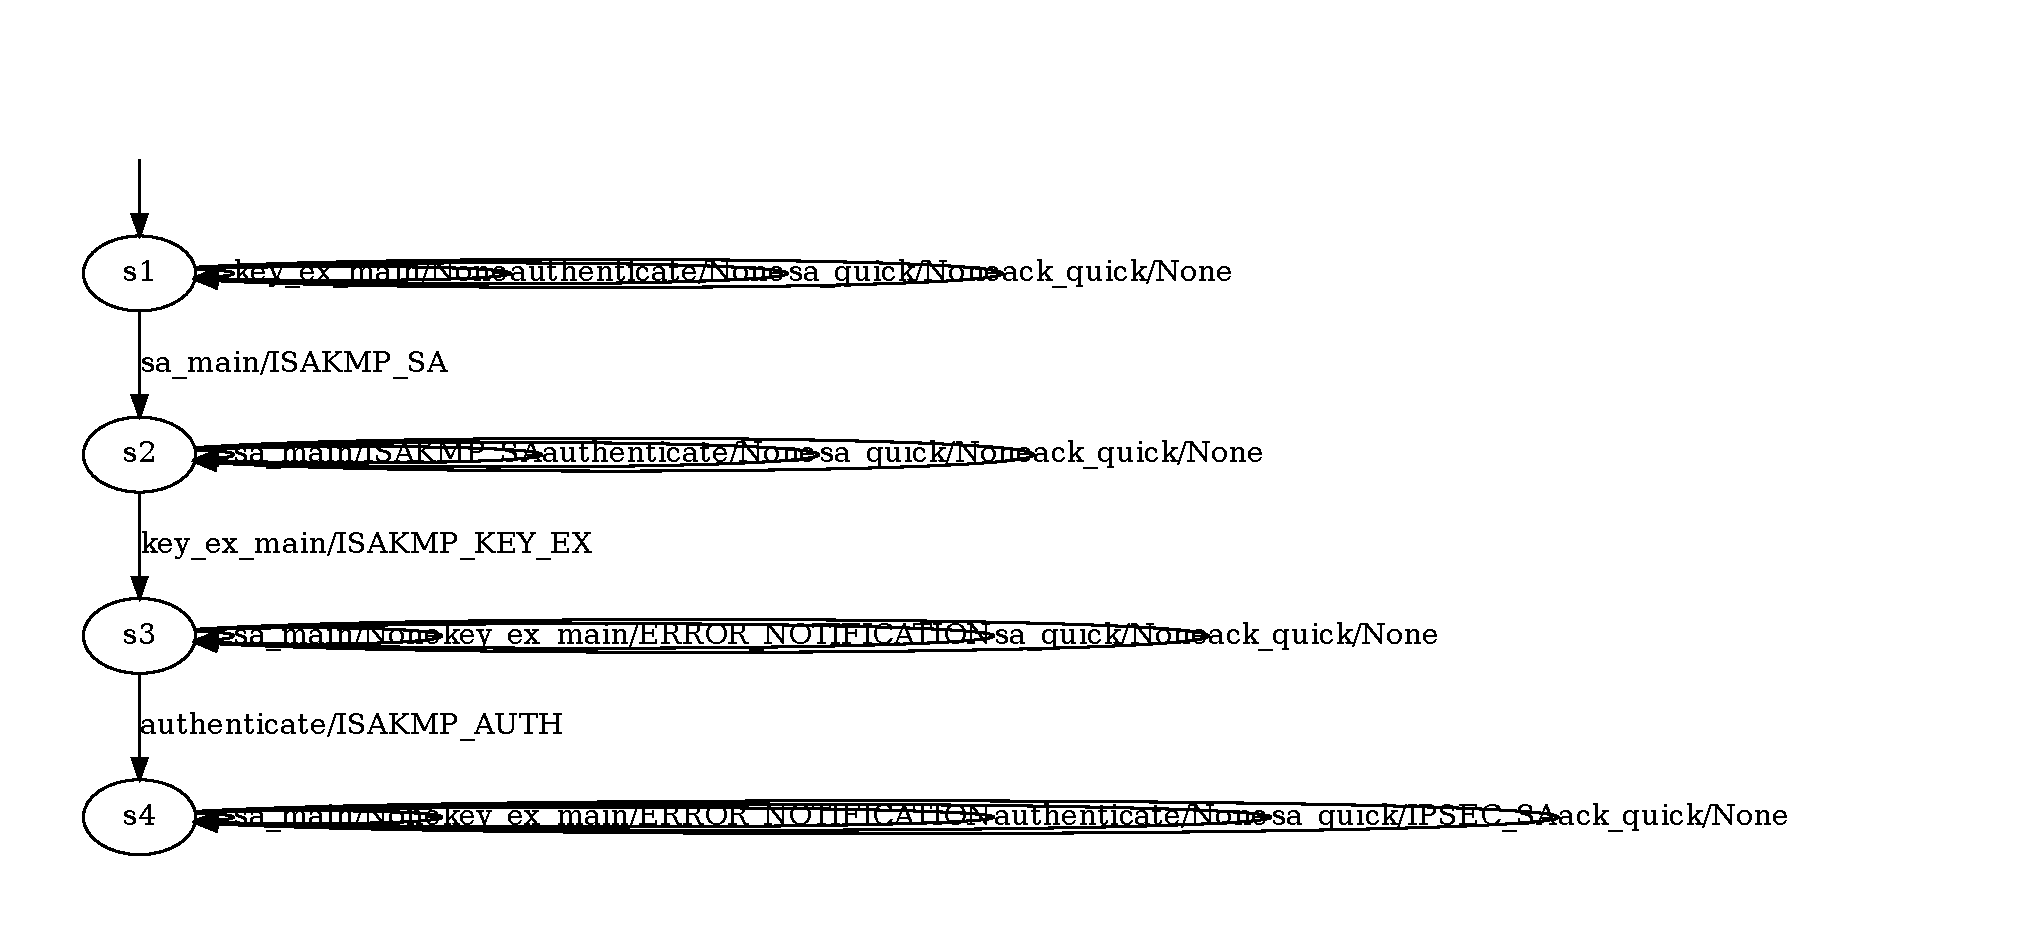
\includegraphics[height=0.9\textheight, trim={8em 0 0 0}]{models/LearnedModelLibreSimple.pdf}
\end{frame}

\begin{frame}{libreswan Fuzzing Reference (Simplified)}
	\vspace{-4em}
	\centering
	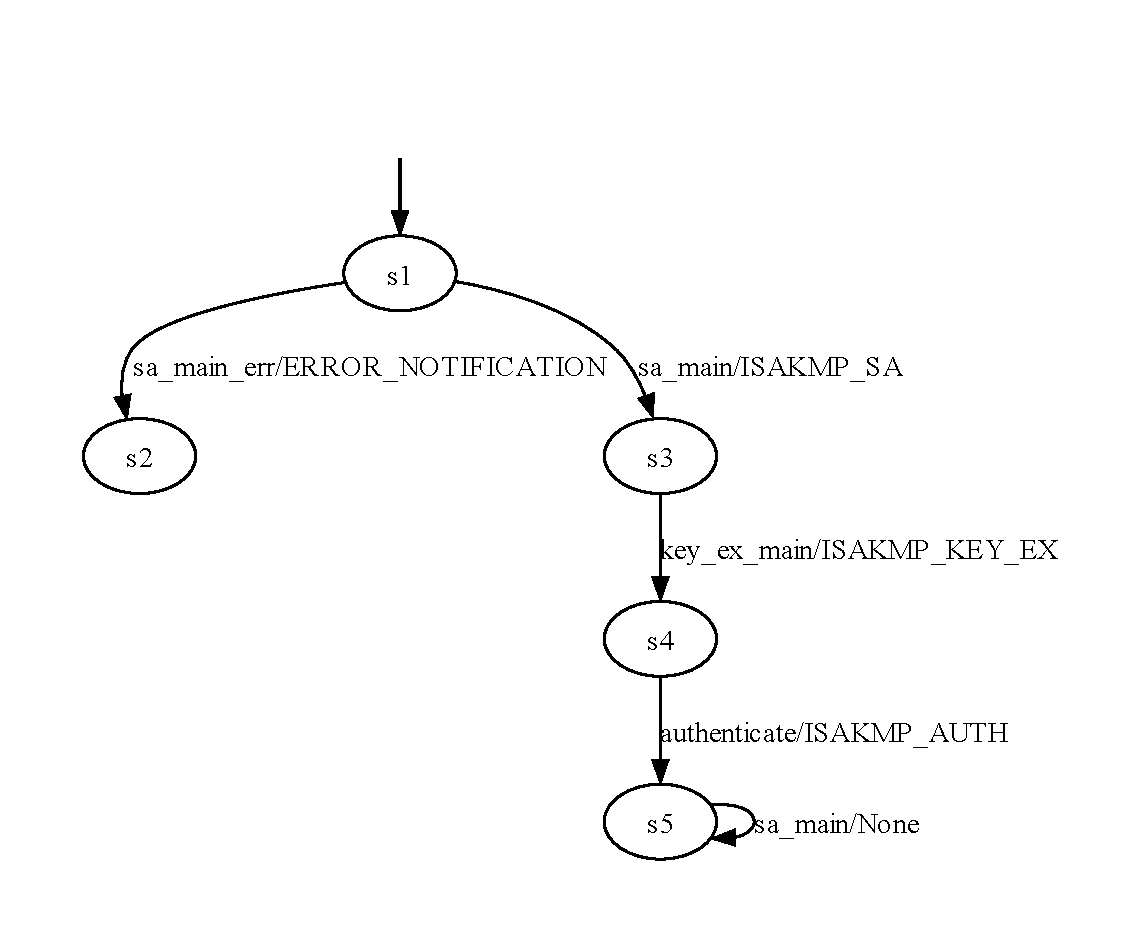
\includegraphics[height=1.0\textheight, trim={8em 0 0 0}]{models/LearnedModelLibreReference}
\end{frame}

\iffalse
	\begin{frame}{Retransmission Sample 1}
		\vspace{-2.7em}
		\centering
		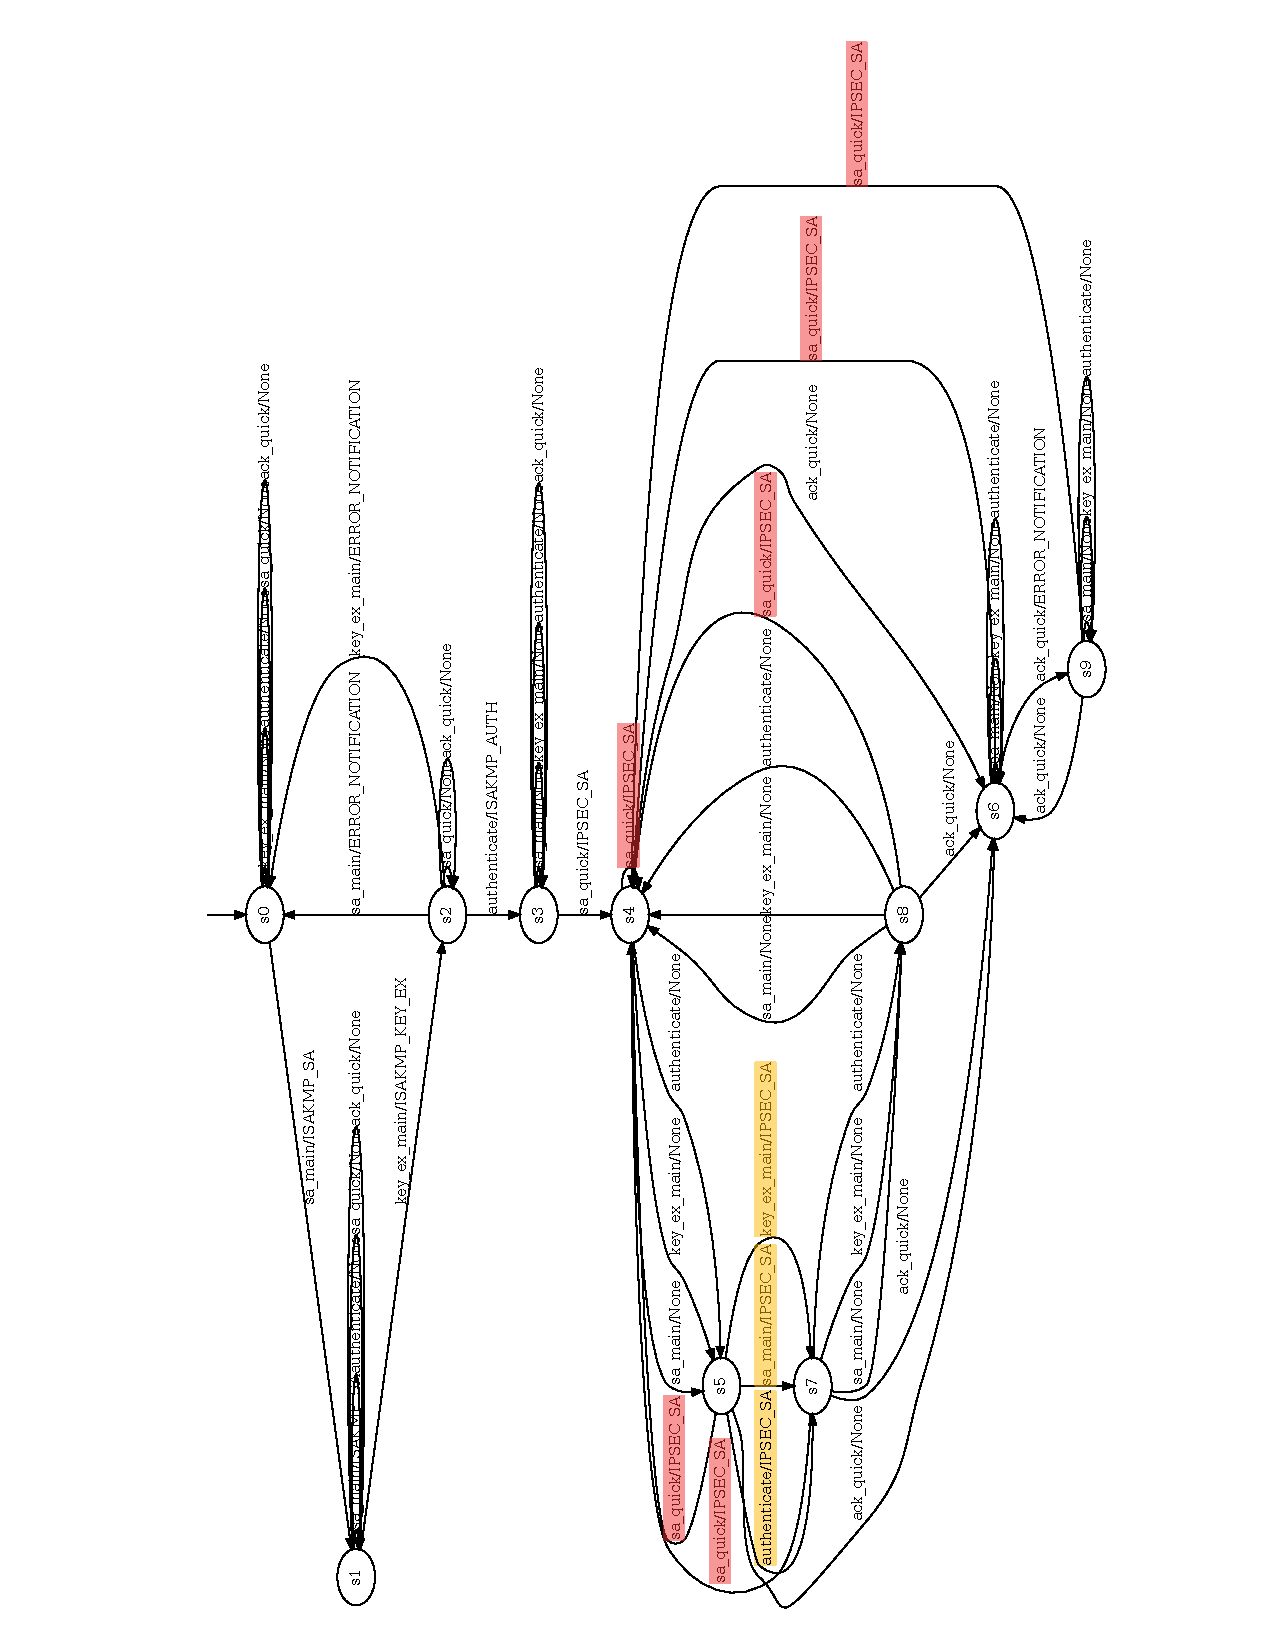
\includegraphics[height=1.45\textheight, angle=270, trim={8em 0 0 0},clip]{models/retransmissions/retrans_case1_lstar}
	\end{frame}
	
	\begin{frame}{Retransmission Sample 2}
		\vspace{-2.7em}
		\centering
		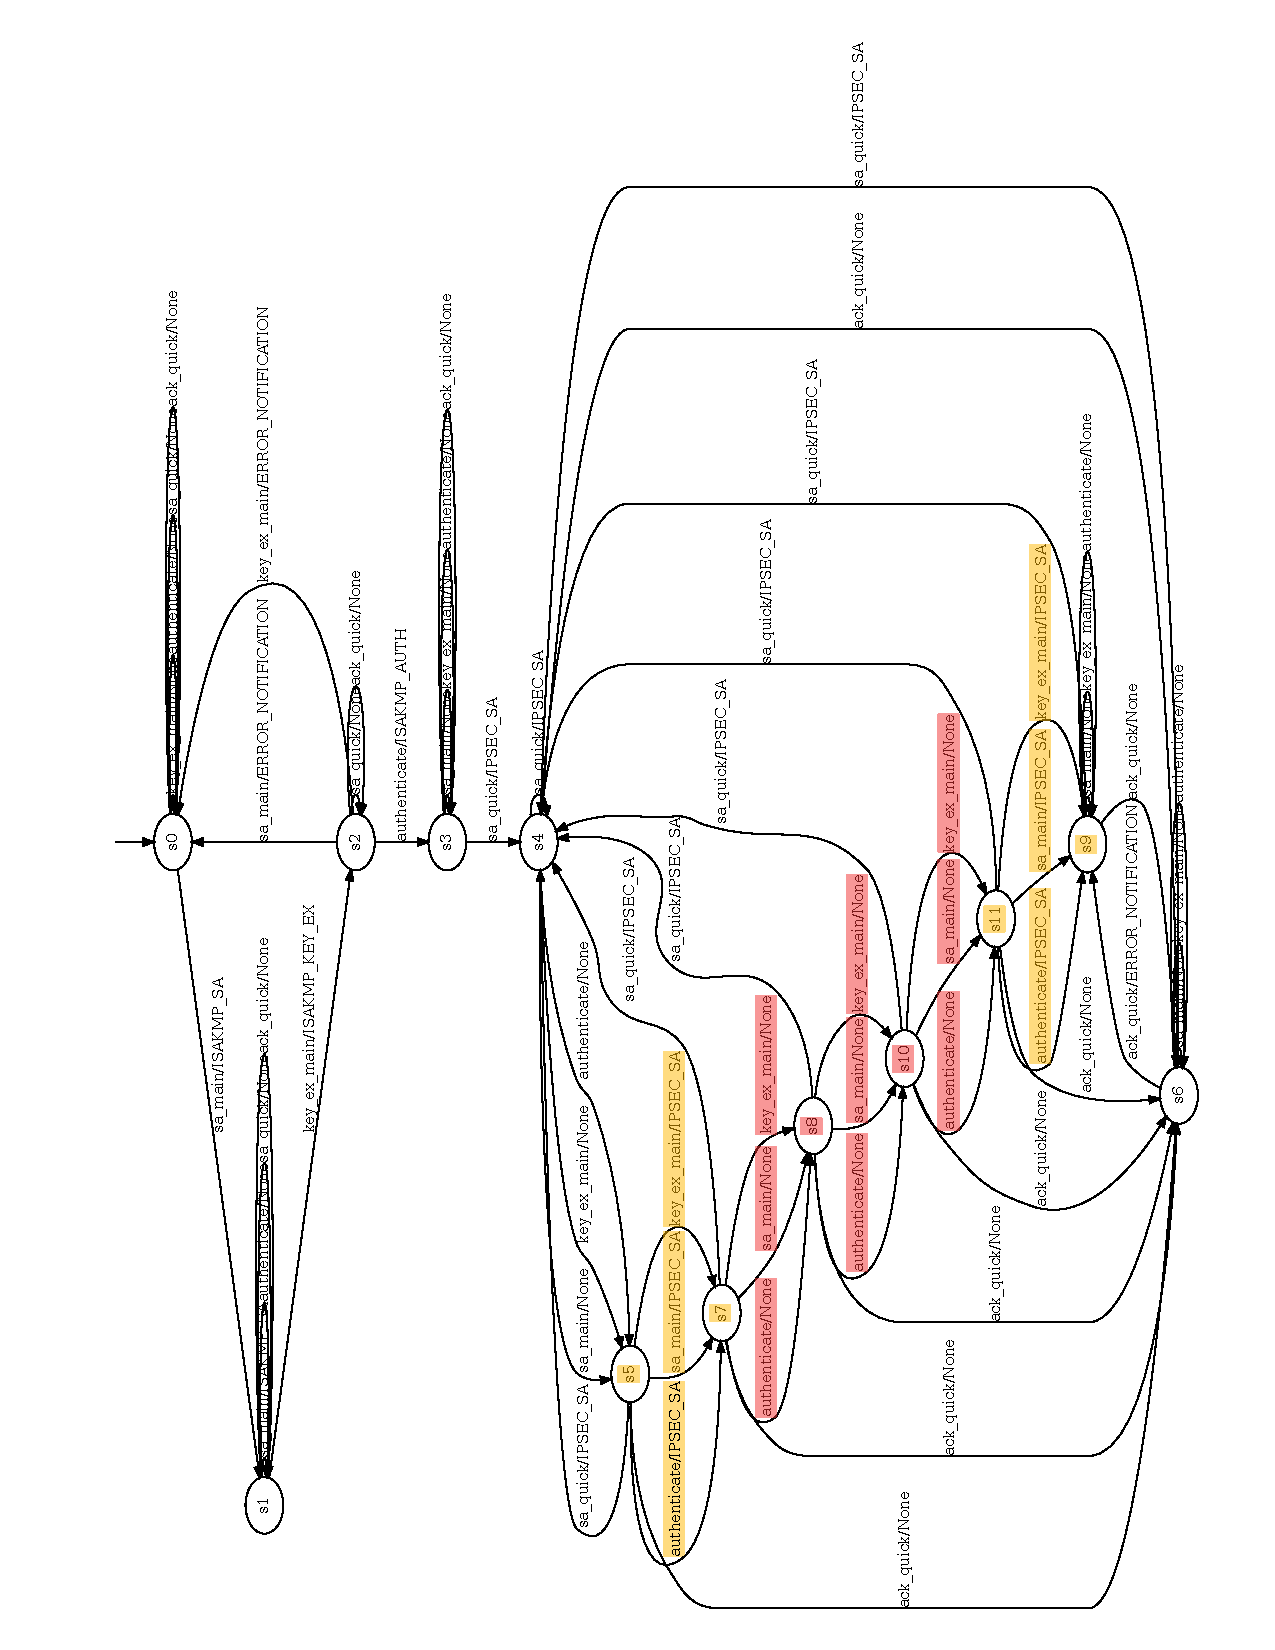
\includegraphics[height=1.2\textheight, angle=270, trim={4em 0 0 0},clip]{models/retransmissions/retrans_case2_lstar}
	\end{frame}
\fi
\section{Fuzzing}

%TODO remove?
\begin{frame}{Fuzzing Overview}
	\vspace{-1.5em}
	\begin{itemize}
		\item Software testing technique
		\pause
		\item Random / unexpected input
		\pause
		\item Categorization:
			\begin{itemize}
				\item Data generation
				\pause
				\item Access to SUT information
			\end{itemize}
	\end{itemize}
\end{frame}

%mention is a software testing technique --> random / unexpected inputs --> SUT
\begin{frame}{Fuzzing Setup - Generic}
	\vspace{-1.2em}
	\centering
	\scalebox{0.6}{
		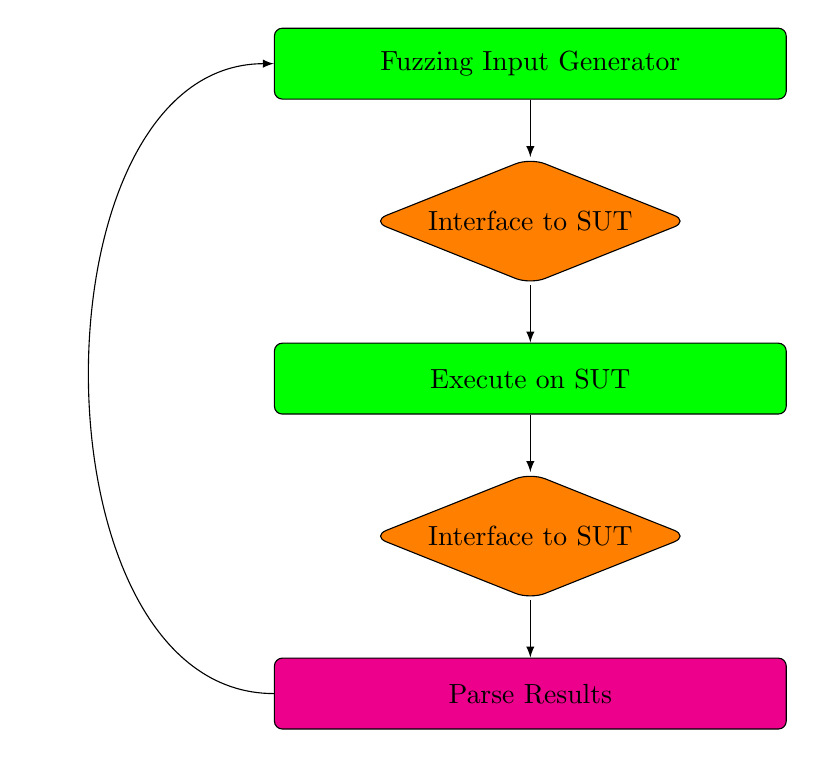
\begin{tikzpicture}
			\node (0) at (0, 8) [draw, rounded corners=0.1cm, fill=green, minimum width=3cm,minimum height=0.9cm, minimum width=6.5cm] {Fuzzing Input Generator};
			\node (1) at (0, 6) [diamond,aspect=2.5,draw, rounded corners=0.2cm, fill=orange] {Interface to SUT};
			\node (2) at (0, 4) [draw, rounded corners=0.1cm, fill=green, minimum width=3cm,minimum height=0.9cm, minimum width=6.5cm] {Execute on SUT};
			\node (3) at (0, 2) [diamond,aspect=2.5,draw, rounded corners=0.2cm, fill=orange]{Interface to SUT};
			\node (4) at (0, 0) [draw, rounded corners=0.1cm, fill=magenta, minimum width=3cm,minimum height=0.9cm, minimum width=6.5cm] {Parse Results};
			
			\draw[-latex] (0) to (1);
			\draw[-latex] (1) to (2);
			\draw[-latex] (2) to (3);
			\draw[-latex] (3) to (4);
			\draw[-latex] (4.west) to[out=180, in=180] (0.west);
		\end{tikzpicture}
	}
\end{frame}

% why input sequences? --> because states locked behind preconditions, guarantees same state each test

\begin{frame}{Fuzzing Setup - Our Approach}
	\vspace{-1.2em}
	\centering
	\scalebox{0.6}{
		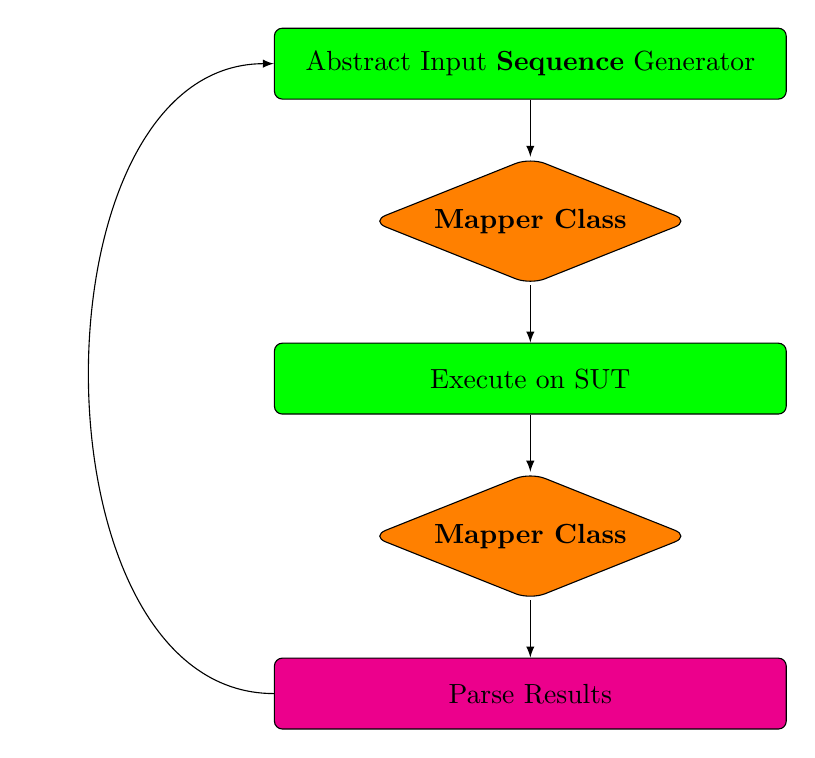
\begin{tikzpicture}
			\node (0) at (0, 8) [draw, rounded corners=0.1cm, fill=green, minimum width=3cm,minimum height=0.9cm, minimum width=6.5cm] {Abstract Input \textbf{Sequence} Generator};
			\node (1) at (0, 6) [diamond,aspect=2.5,draw, rounded corners=0.2cm, fill=orange] {\textbf{Mapper Class}};
			\node (2) at (0, 4) [draw, rounded corners=0.1cm, fill=green, minimum width=3cm,minimum height=0.9cm, minimum width=6.5cm] {Execute on SUT};
			\node (3) at (0, 2) [diamond,aspect=2.5,draw, rounded corners=0.2cm, fill=orange]{\textbf{Mapper Class}};
			\node (4) at (0, 0) [draw, rounded corners=0.1cm, fill=magenta, minimum width=3cm,minimum height=0.9cm, minimum width=6.5cm] {Parse Results};
			
			\draw[-latex] (0) to (1);
			\draw[-latex] (1) to (2);
			\draw[-latex] (2) to (3);
			\draw[-latex] (3) to (4);
			\draw[-latex] (4.west) to[out=180, in=180] (0.west);
		\end{tikzpicture}
	}
\end{frame}

%how do we detect new states? --> iffy, more so just detect new behaviour via the state machine
\begin{frame}{Detecting new behavior}
	\vspace{-1.2em}
	\scalebox{0.8}{
		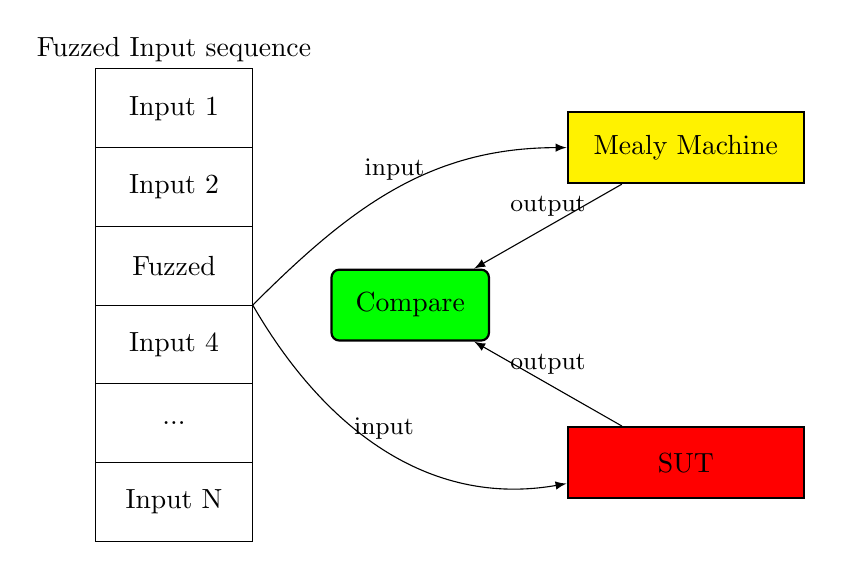
\begin{tikzpicture}
			\node (title) at (1,6.25) {Fuzzed Input sequence};
			\node (0) at (0, 6) {};
			\node (1) at (0, 5) {};
			\node (2) at (0, 4) {};
			\node (3) at (0, 3) {};
			\node (4) at (0, 2) {};
			\node (5) at (0, 1) {};
			\node (6) at (0, 0) {};
			\node (7) at (2, 0) {};
			\node (8) at (2, 1) {};
			\node (9) at (2, 2) {};
			\node (10) at (2, 3) {};
			\node (11) at (2, 4) {};
			\node (12) at (2, 5) {};
			\node (13) at (2, 6) {};
			
			\node (sut) at (7.5, 1) [draw,thick,minimum width=3cm,minimum height=0.9cm, fill=red] {SUT};
			\node (26) at (1, 2.5) {Input 4};
			\node (27) at (1, 5.5) {Input 1};
			\node (28) at (1, 4.5) {Input 2};
			\node (29) at (1, 3.5) {Fuzzed};
			\node (30) at (1, 1.5) {...};
			\node (31) at (1, 0.5) {Input N};
			\node (32) at (6, 6) {};
			\node (33) at (6, 4) {};
			\node (34) at (9, 4) {};
			\node (35) at (9, 6)  {};
			\node (sm) at (7.5, 5) [draw,thick,minimum width=3cm,minimum height=0.9cm, fill=yellow] {Mealy Machine};
			\node (37) at (2, 3) {};
			\node (39) at (6, 0.5) {};
			\node (40) at (6, 4.75) {};
			\node (comp) at (4, 3) [draw,thick,minimum width=2cm,minimum height=0.9cm,rounded corners=.1cm, fill=green] {Compare};
			\node (42) at (6, 1.5) {};
			
			\draw [in=180, out=0] (0.center) to (13.center);
			\draw (0.center) to (1.center);
			\draw (1.center) to (2.center);
			\draw (2.center) to (3.center);
			\draw (3.center) to (4.center);
			\draw (4.center) to (5.center);
			\draw (5.center) to (6.center);
			\draw (6.center) to (7.center);
			\draw (7.center) to (8.center);
			\draw (8.center) to (9.center);
			\draw (9.center) to (10.center);
			\draw (10.center) to (11.center);
			\draw (11.center) to (12.center);
			\draw (12.center) to (13.center);
			\draw (1.center) to (12.center);
			\draw (2.center) to (11.center);
			\draw (3.center) to (10.center);
			\draw (4.center) to (9.center);
			\draw (5.center) to (8.center);
			\draw[-latex] (37.center) to [out=45,in=180] node[pos=0.5, above, font=\small]{input} (sm);
			\draw[-latex](37.center) to [out=300,in=190] node[pos=0.5, above, font=\small]{input} (sut);
			\draw[-latex] (sm) -- node[pos=0.5, above, font=\small]{output} (comp);
			\draw[-latex] (sut) -- node[pos=0.5, above, font=\small]{output} (comp);
		\end{tikzpicture}	
	}
\end{frame}

%what guarantees do we make for coverage? --> with filtering method, good coverage, for the others, depends on how effective the search is, but that is its goal
%other improvements? --> mapper class adaptations, this would get very difficult if we kept state of multiple connections

\iffalse
\begin{frame}{Input Sequence Generation - Random}
	\vspace{-1.5em}
	\begin{itemize}
		\item Random abstract inputs %of the input alphabet
		\pause
		\item Our baseline
		\pause
		\item Inefficient and ineffective
	\end{itemize}
\end{frame}
\fi
% completely random is very bad, as the protocol itself is stateful and split into two phases. If left to completely random, we likely never reach phase 2 within a reasonable 
% timeframe --> filtering base, reuse old input sequences from learning --> have to filter them cause there are a loot --> try and choose meaningful ones that lead to new info
% pre-fuzz them and filter out those that dont seem interesting, then fuzz only one input per sequence that is known to be interesting

\begin{frame}{Input Sequence Generation - Filtering}
	\vspace{-1.5em}
	\begin{columns}[T]
		\begin{column}{0.5\textwidth}
				\begin{itemize}
				\item Reuse input sequences from model learning %~220
				\item Automatic Filtering %minimal fuzzing
				\item Manual Filtering %removing duplicates --> 55 at the end
			\end{itemize}
		\end{column}
		\begin{column}{0.5\textwidth}
			\scalebox{0.5}{
				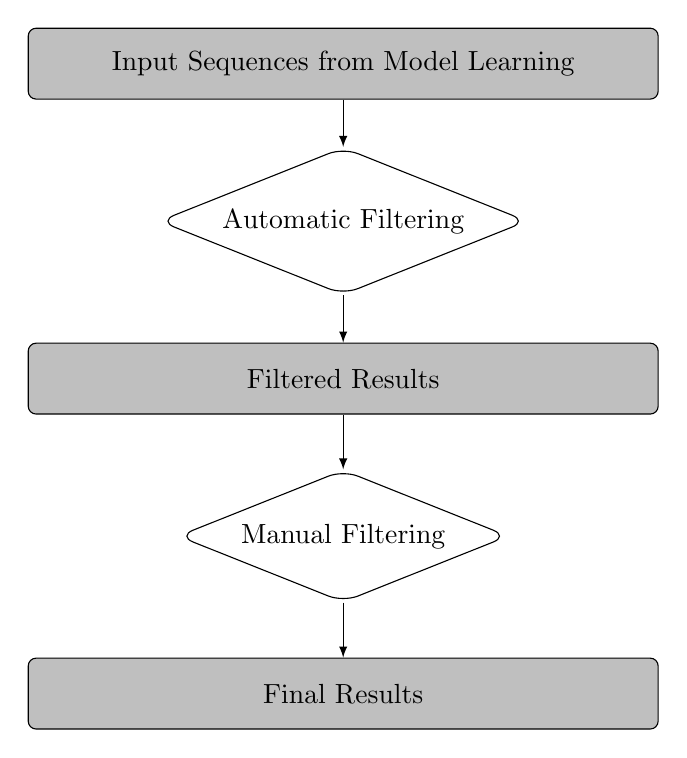
\begin{tikzpicture}
					\node (0) at (0, 8) [draw, rounded corners=0.1cm, fill=lightgray, minimum width=3cm,minimum height=0.9cm, minimum width=8cm] {Input Sequences from Model Learning};
					\node (1) at (0, 6) [diamond,aspect=2.5,draw, rounded corners=0.2cm] {Automatic Filtering};
					\node (2) at (0, 4) [draw, rounded corners=0.1cm, fill=lightgray, minimum width=3cm,minimum height=0.9cm, minimum width=8cm] {Filtered Results};
					\node (3) at (0, 2) [diamond,aspect=2.5,draw, rounded corners=0.2cm]{Manual Filtering};
					\node (4) at (0, 0) [draw, rounded corners=0.1cm, fill=lightgray, minimum width=3cm,minimum height=0.9cm, minimum width=8cm] {Final Results};
					
					\draw[-latex] (0) to (1);
					\draw[-latex] (1) to (2);
					\draw[-latex] (2) to (3);
					\draw[-latex] (3) to (4);
				\end{tikzpicture}
			}
		\end{column}
	\end{columns}
\end{frame}

% greater or equal stopping criteria
\begin{frame}{Input Sequence Generation - Search}
	\vspace{-1.5em}
	\begin{columns}[T]
		\begin{column}{0.4\textwidth}
			\begin{itemize}
				\item Single input sequence
				\item Search-based 
				\item Fitness function
			\end{itemize}
		\end{column}
		\begin{column}{0.6\textwidth}
			\begin{equation}f_\mathrm{seq} = \sum_{0}^{n-1} \frac{b_\mathrm{new}}{n} \frac{s_\mathrm{visited}}{s_\mathrm{total}} \end{equation}
		\end{column}
	\end{columns}
\end{frame}

% show reward function?

\begin{frame}{Input Sequence Generation - Genetic}
	\vspace{-1.5em}
	\begin{itemize}
		\item Pool of populations
		\item Mutation operations
	\end{itemize}
	\centering
	\vspace{-1em}
	\scalebox{0.7}{
		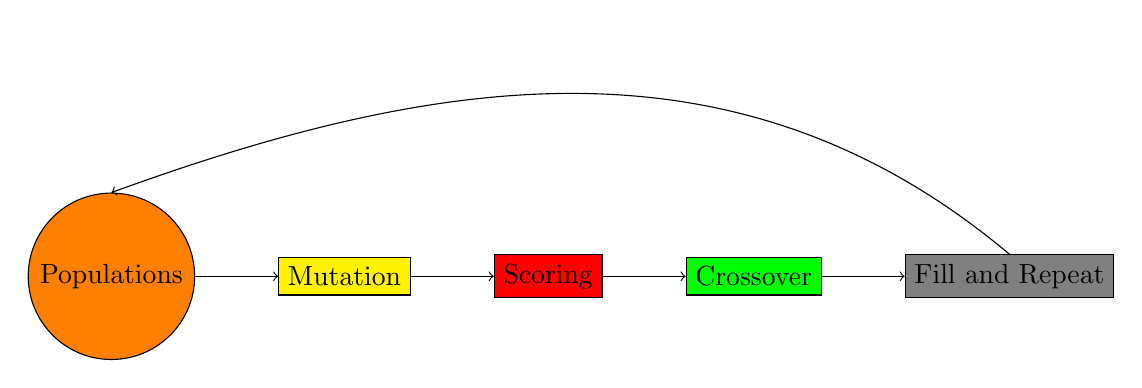
\begin{tikzpicture}[]
			% Define the nodes
			\node (start) [circle, draw, fill=orange] {Populations};
			\node (input) [rectangle, draw, right=3em of start, fill=yellow] {Mutation};
			\node (process) [rectangle, draw, right=3em of input, fill=red] {Scoring};
			\node (output) [rectangle, draw, right=3em of process, fill=green] {Crossover};
			\node (stop) [rectangle, draw, right=3em of output, fill=gray] {Fill and Repeat};
			% Connect the nodes
			\draw [->] (start) -- (input);
			\draw [->] (input) -- (process);
			\draw [->] (process) -- (output);
			\draw [->] (output) -- (stop);
			\draw [->] (stop.north) to [out=140,in=20] (start.north);
		\end{tikzpicture}
	}	
\end{frame}

\iffalse
% note that filtering is an average over all their input sequences
% note that all non-baseline methods discovered all the findings
\begin{frame}{Input Sequence Generation - Comparison}
	\centering
	\begin{tabular}{|l|l|}
		\hline
		\rowcolor[HTML]{EFEFEF} 
		\textbf{Method} & \textbf{Fitness Score}  \\ \hline
		Baseline (8)              	&  0.0542     \\ \hline
		Baseline (18)              	&  0.392      \\ \hline
		Filtering (avg)             &  1.4712     \\ \hline
		Search              		&  2.8125     \\ \hline
		Genetic              		&  4.7        \\ \hline
	\end{tabular}
\end{frame}



\begin{frame}{Input Sequence Generation}
	\begin{itemize}
		\item Filtering
		\item Search
		\item Genetic
	\end{itemize}
\end{frame}
\fi
%TODO maybe add some nicer hihglighting
\section*{Fuzzing Results}
\begin{frame}[fragile]{Finding -  ISAKMP Length}
	\vspace{-2ex}
	\begin{lstlisting}[]
Fuzzing ISAKMP length field with: b'\xff\x00\x00\x00'
Input sequence: ['sa_main_fuzz', 'key_ex_main', 'authenticate', ...]

$sa_main_fuzz
$key_ex_main

**********
Expected: ERROR_NOTIFICATION | Received: ISAKMP_SA
Expected: None | Received: ISAKMP_KEY_EX
**********
	\end{lstlisting}
\end{frame}

% the corresponding ID? --> TODO check is that the name --> think initiator cookie? becomes unuseable
\begin{frame}{Finding - libreswan Deadlock}
	\vspace{-4em}
	\centering
	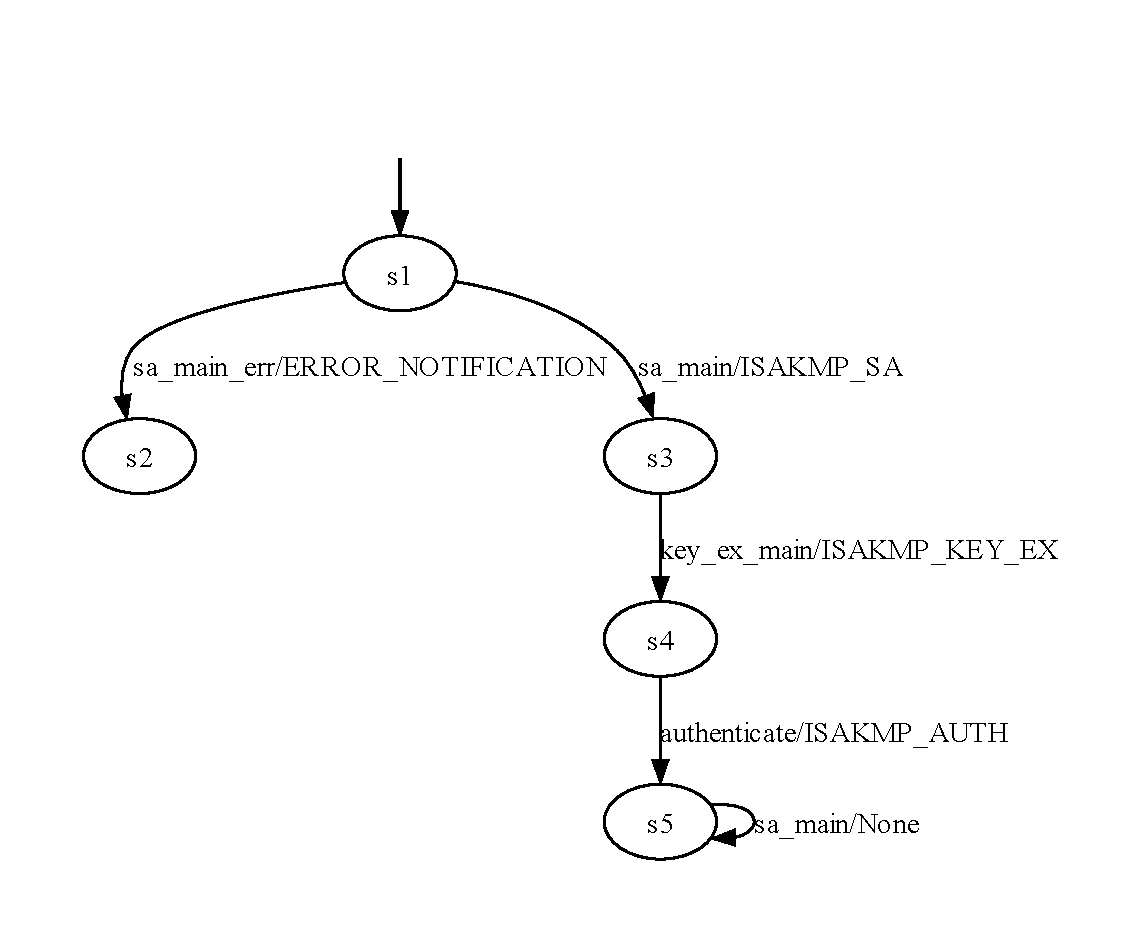
\includegraphics[height=1.0\textheight, trim={8em 0 0 0}]{models/LearnedModelLibreReference}
\end{frame}

% wireshark shows SA response defaulting to PSK auth
% brief injection of arbitrary values (length limited) into runtime memory + messing up of the state machine
\begin{frame}[fragile]{Finding - StrongSwan Authentication}
	\vspace{-2ex}
	\begin{lstlisting}[]
		Fuzzing SA Transform with: [..., ('Authentication', 'FUZZED_VALUE'), ...]
		
		Run: [..., 'sa_main_fuzz', ...]
		
		$sa_main_fuzz
		
		**********
		Expected: ERROR_NOTIFICATION | Received: ISAKMP_SA
		**********
	\end{lstlisting}
\end{frame}

\section*{}

\begin{frame}{Conclusion}
	\vspace{-1.5em}
	\begin{itemize}
		\item Learned models of popular IPsec implementations
		\item Fuzzing revealed several deviations from specifications
		\item Future work:
		\pause
		\begin{itemize}
			\item Mapper class improvements
			\item Additional input-sequence / fuzz-data generation methods
			\item Fuzz with more resources
		\end{itemize}
	\end{itemize}
\end{frame}
% future work expand the mapper class to handle multiple simultaneous connections and work well with delete, support additional features
% additional methods of input sequence generation --> better reward functions / mutations
% more resources
\end{document}
